\documentclass[11pt]{article}
\usepackage[margin=2.2cm]{geometry}
\usepackage{graphicx, booktabs, hyperref, float}
\graphicspath{{../figures/}}
\title{Run 224489: Cross-Wiring Fix Confirmed, First Plastic-MIP Calibration
       from Liquid-Scintillator Triples,\\ and the Second Plastic HV Scan\\
       \large n\_TOF EAR2 X17 campaign, run 224489 (July 17, 2026)}
\author{Dylan Neff \\[0.5ex] {\small analysis and document prepared with Claude (Anthropic AI assistant)}}
\date{July 18, 2026}

\begin{document}
\maketitle

\begin{abstract}
Run 224489 (1750 bunches, EAR2) is the first run with the liquid scintillators
(LIQ) in the readout, the first after the A/D cabling fix, and the first with
the plastics on a linear fan-in/fan-out (FIFO) instead of the BNC-T split; it
also repeats the nine-step plastic HV ladder of run 224466. Five headline
results. (1)~The cross-wiring fix is confirmed: the $\pm4$\,ns equal-amplitude
duplication band on arms A/D is gone (flagged fractions $\leq$4\%, the B-arm
control level, vs.\ 23--31\% before), all four arms now show equal wall--plastic
coincidence excess, and A/D display clean MIP bumps with no veto --- the
standing A/D deficit was the cabling. (2)~Triple coincidences
WAL$\times$PSS$\times$LIQ select through-going particles and yield the
\emph{first plastic-MIP calibration}: MIP (linear-space MPV) amplitudes at
nominal HV span 3.3\,mV (DR) to 10.3\,mV (AL), i.e.\ 0.65--2.05\,mV/MeV
against the expected 5.05\,MeV deposit in 2.5\,cm of PVT; the DR and BL MIPs
sit below the recommended 4.9\,mV trigger threshold. The extraction is
validated against the no-MIP-selection coincident median: both follow the
same gain power law, the MIP sitting a factor $\sim$10 below. (3)~The FIFO recovers only
$\times1.40$ (fleet geometric mean; 1.13--1.65 per PMT) rather than the naive
$\times2$. (4)~The liquids are timed in: every arm shows a sharp LIQ
coincidence peak, the LIQ pulse leading the plastic by $\sim$30\,ns; and the
suspected LIQ gain gradient is real --- a 1.5--2$\times$ amplitude variation
along the vessel axis, higher near the PMT, whose direction flips with the
surveyed vessel orientation. (5)~All 64 wall--plastic time offsets shifted by
a single common $-22.27$\,ns (rms 0.22\,ns), while the $-60$\,ns satellite
bump kept its \emph{absolute} position and grew to 19--34\% of the main peak:
it is not a plastic-cable reflection and warrants a scope check at the FIFO.
A new HV-equalization table supersedes the run-224466 one.
\end{abstract}

\section{Run overview and hardware changes}
Run 224489 was taken 2026-07-17 (17:39--19:17 local) during the second
plastic HV scan (\texttt{plastic\_scan\_2}): the same nine-step ladder as
run 224466 --- pass~1 at 1600$\to$1200\,V in 100\,V steps, pass~2 at
1550$\to$1250\,V --- merged into a uniform 50\,V grid, followed by a
$\sim$12\,min post-scan window at the per-channel nominal HV
(AL~1325, AR~1275, BL~1325, rest 1300\,V). Four things changed since 224466:

\begin{enumerate}
\item \textbf{Cabling fix}: the crossed/duplicated same-side channels on arms
      A and D (identified after runs 224404/224460) were re-cabled.
\item \textbf{FIFO}: the plastic signals now reach DAQ and trigger through a
      linear fan-in/fan-out instead of a passive BNC-T split, adding
      $\sim$16\,ns of cable and (naively) a factor 2 in amplitude.
\item \textbf{Liquid scintillators}: trees LIQA--D (one channel each) appear
      for the first time, with 5.3\,M (C) to 21.6\,M (B) hits.
\item \textbf{SiPM flash gating ON for the whole run} (no mid-run boundary,
      unlike 224466).
\end{enumerate}

Processing used R.~Mucciola's new PSA (\texttt{UserInput\_2026\_EAR2\_X17.h},
pulse-shape fitting for WALL and LIQ). Data quality is excellent: no SiPM-wall
outage (0 of 1750 bunches, vs.\ 46\% lost in 224404), $\gamma$-flash at
11.62\,$\mu$s on all arms, and all 44 channels alive. All results
below use beam-on, wall-active bunches and, for spectra, hits more than
0.1\,ms after the $\gamma$-flash. Bunches are assigned to HV steps by matching
PKUP wall-clock times against the CAEN HV log (Fig.~\ref{fig:timeline}).

\begin{figure}[H]\centering
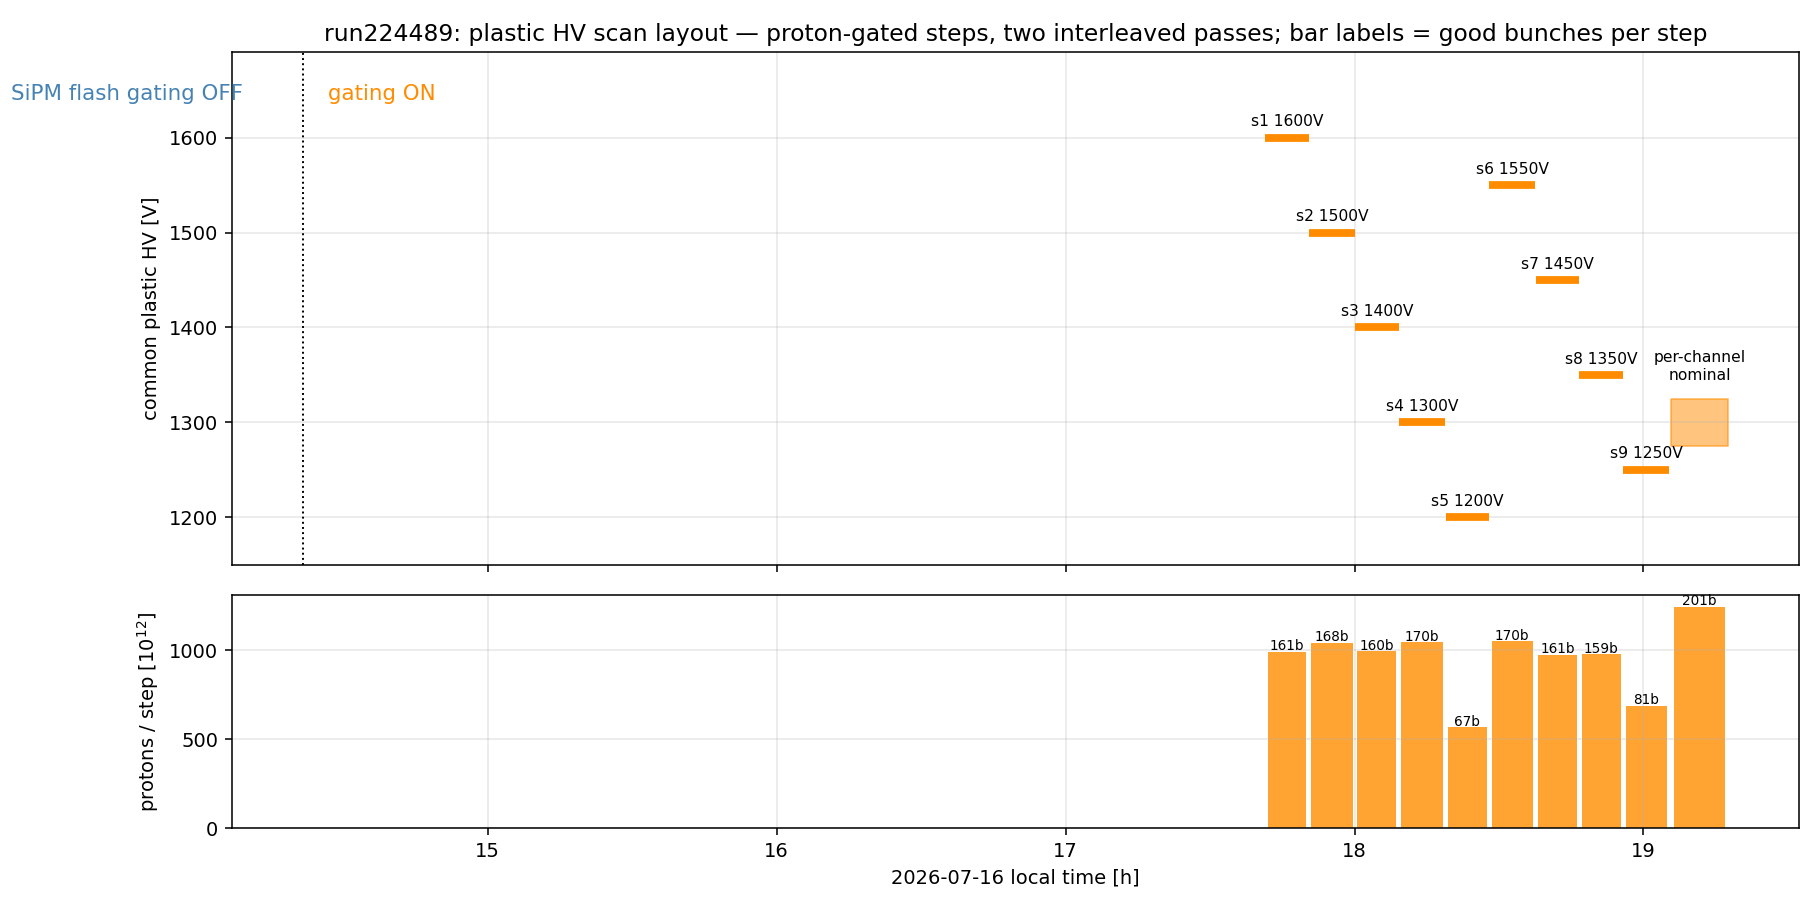
\includegraphics[width=.9\textwidth]{12_hv_scan/scan_timeline.png}
\caption{HV staircase vs.\ wall clock with delivered protons per step. The
run has no usable pre-scan window (the first raw file closed one minute
before the scan started); the post-scan \emph{end\_nominal} window
(19:05--19:17) provides the operating-point reference.}
\label{fig:timeline}
\end{figure}

\section{The cross-wiring fix is confirmed; the A/D question is closed}
\label{sec:wiring}
In runs 224404/224460, arms A and D showed 6--8$\times$ fewer true
wall--plastic coincidences than B/C and no MIP bump, and a duplication veto
study found 23--31\% of hits on the affected channels accompanied by an
equal-amplitude partner one group over within $\pm4$\,ns
(Table~\ref{tab:dup}). In run 224489 every one of those signatures is gone:

\begin{table}[H]\centering\small
\begin{tabular}{lcccccccc}
\toprule
flagged fraction (signal pairs) & ch1 & ch2 & ch3 & ch4 & ch5 & ch6 & ch7 & ch8\\
\midrule
arm A, run224460 & 0.012 & 0.029 & 0.029 & 0.047 & \textbf{0.306} & 0.049 & \textbf{0.325} & 0.026\\
arm A, run224489 & 0.011 & 0.026 & 0.026 & 0.042 & 0.036 & 0.044 & 0.024 & 0.023\\
\midrule
arm D, run224460 & 0.027 & \textbf{0.311} & 0.043 & \textbf{0.265} & \textbf{0.308} & 0.043 & \textbf{0.343} & 0.021\\
arm D, run224489 & 0.024 & 0.021 & 0.039 & 0.039 & 0.038 & 0.038 & 0.025 & 0.019\\
\midrule
arm B (control), run224489 & 0.011 & 0.008 & 0.016 & 0.011 & 0.029 & 0.024 & 0.026 & 0.024\\
\bottomrule
\end{tabular}
\caption{Duplication-veto flagged fractions. The 23--34\% bands on the
crossed A/D channels (bold) collapse to the B-arm control level after the fix.}
\label{tab:dup}
\end{table}

Simultaneously, the wall--plastic excess is now equal on all four arms
(1.79/1.71/1.81/1.75\,M on A/B/C/D within $\pm$10\,ns) and the A/D coincident
wall spectra show clean MIP peaks with \emph{no} veto applied
(Fig.~\ref{fig:dupveto}). The conclusion is loud and simple: \textbf{the A/D
coincidence deficit was the cabling, and it is fixed.} The wall-MIP
calibration now covers all four arms.

\begin{figure}[H]\centering

\includegraphics[width=\textwidth]{run224489/autopsy/dup_veto_spectra.png}
\caption{Run 224489 duplication-veto autopsy: sideband-subtracted coincident
wall spectra per channel, as-is (colored) vs.\ veto survivors (black dashed).
Unlike 224460, the two are nearly identical everywhere and every channel
shows a MIP bump.}
\label{fig:dupveto}
\end{figure}

\section{Plastic HV scan: gain laws, FIFO ratio, new equalization}
\subsection{Wall MIP is again immune to the plastic HV}
The channel-summed, sideband-subtracted wall MIP peak moves by at most one
histogram bin ($\pm2.6\%$) on every arm across the full 1200--1600\,V plastic
range (Fig.~\ref{fig:wallmip}) --- reproducing the 224466 result, now
including arm A. The wall energy scale is independent of the plastic
operating point.

\begin{figure}[H]\centering
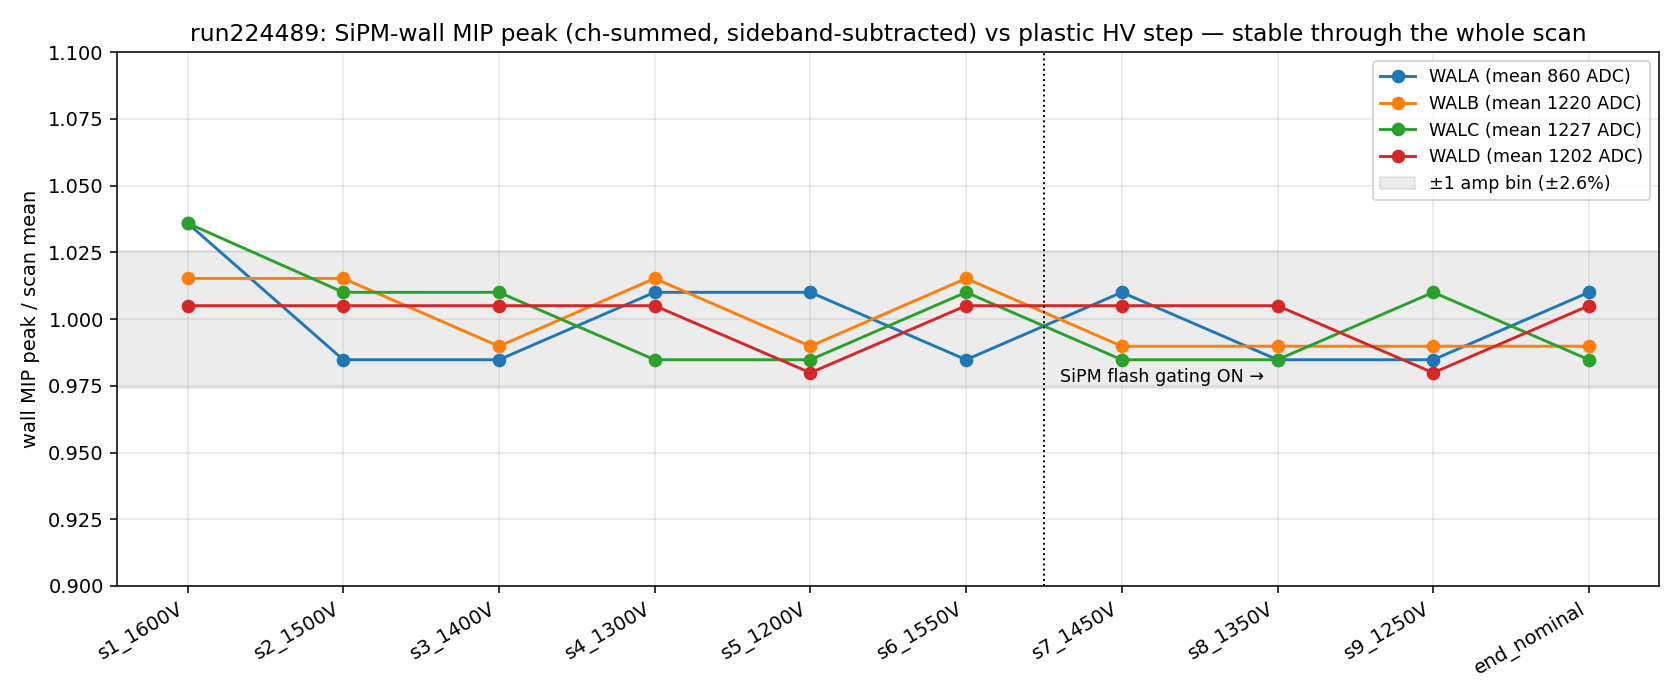
\includegraphics[width=.95\textwidth]{12_hv_scan/wall_mip_stability.png}
\caption{Wall MIP peak position vs.\ plastic HV step, per arm.}
\label{fig:wallmip}
\end{figure}

\subsection{Per-PMT gain power laws}
Wall-tagged, sideband-subtracted plastic medians follow clean power laws
$G\propto V^{n}$ with $n=3.8$--7.1 (Fig.~\ref{fig:gain}), passes consistent.
Two cautionary tales repeat: the \emph{inclusive} medians of PSSB1 and PSSD2
are non-monotonic in $V$ (apparent $n<1$) --- pure threshold bias --- while
their coincident fits are perfectly ordinary ($n=5.2$, $6.4$). Inclusive
medians are not a gain proxy.

\begin{figure}[H]\centering
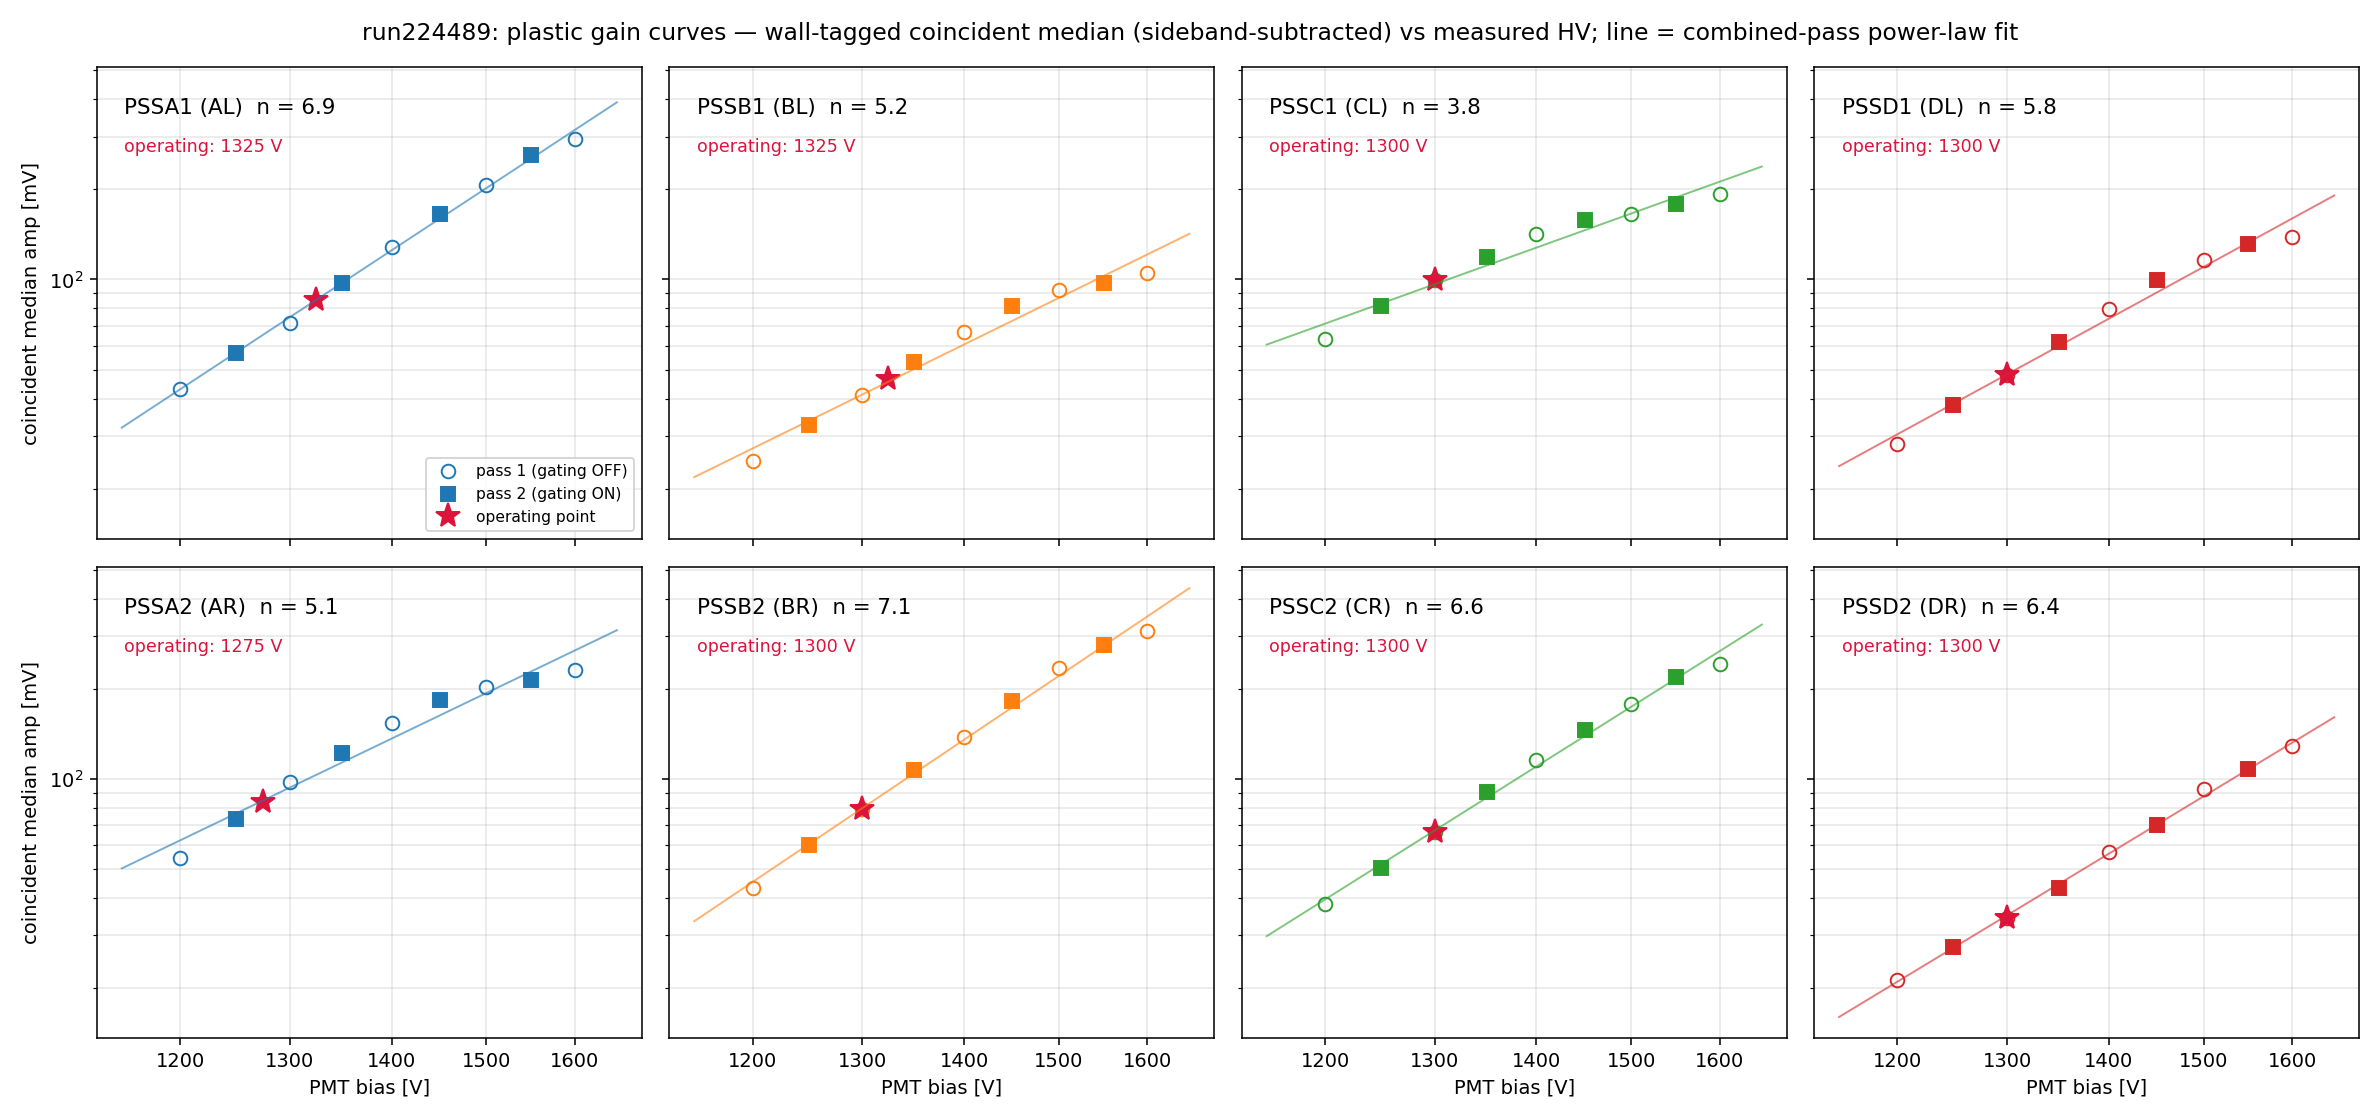
\includegraphics[width=\textwidth]{12_hv_scan/gain_curves.png}
\caption{Coincident-median gain curves per PMT with power-law fits; the red
star marks the operating point in the post-scan window.}
\label{fig:gain}
\end{figure}

\begin{figure}[H]\centering
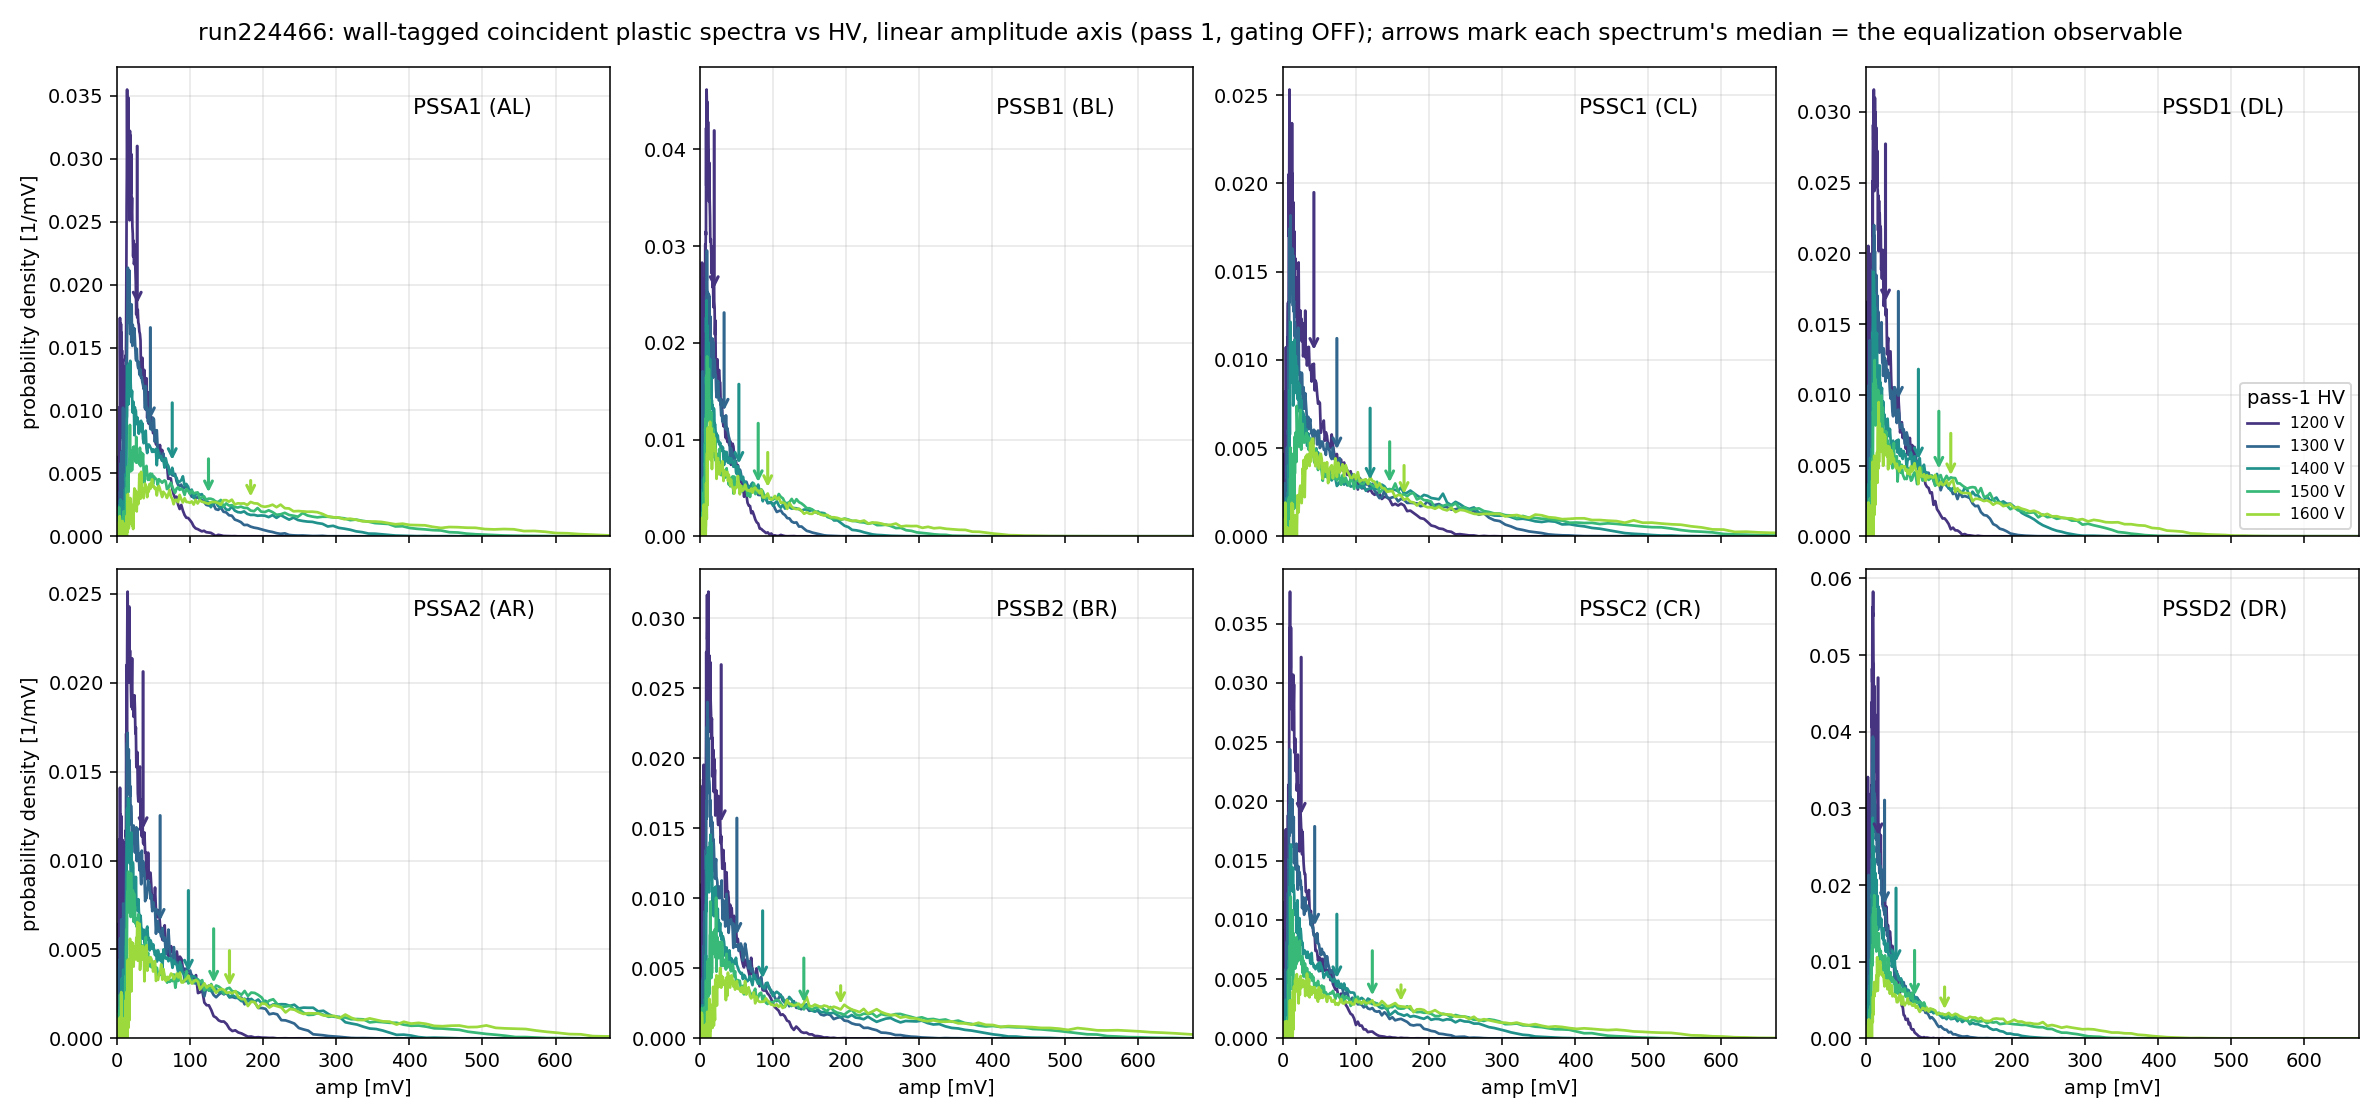
\includegraphics[width=\textwidth]{12_hv_scan/coinc_spectra_linear.png}
\caption{Wall-tagged plastic spectra per step (linear mV axis): the spectral
shape marches coherently with HV.}
\label{fig:coincspec}
\end{figure}

\subsection{The FIFO gain ratio is 1.4, not 2}
Comparing coincident medians at equal HV between 224489 (FIFO) and 224466
(BNC-T split) measures the signal-path change directly
(Fig.~\ref{fig:fifo}). The fleet geometric mean is $\times1.40$, but the
per-PMT values span 1.13 (DL) to 1.65 (AL) and are roughly flat in $V$. The
naive expectation --- removing a passive T halves the signal, so the FIFO
should double it --- is wrong in detail; the FIFO's per-channel drive and the
old T's actual splitting ratio evidently differ channel by channel. Any gain
bookkeeping must use the measured per-PMT ratios, not a global factor 2.

\begin{figure}[H]\centering
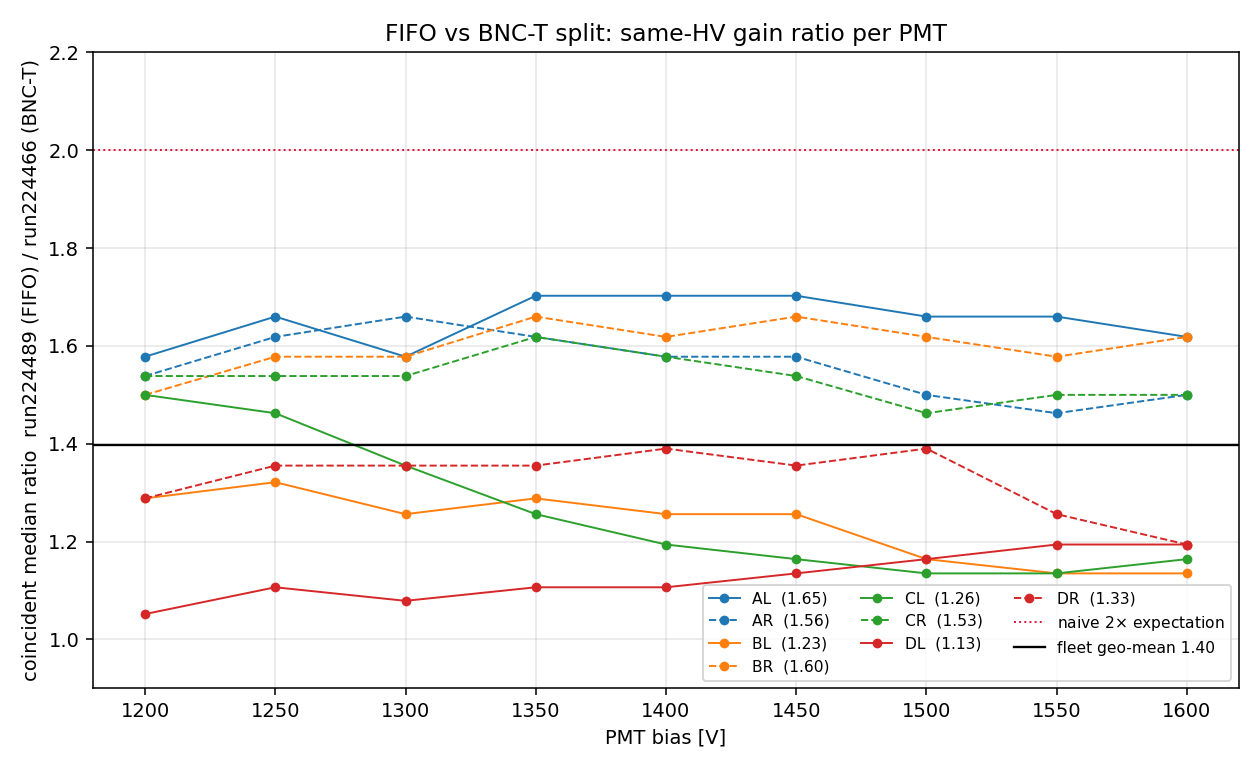
\includegraphics[width=.75\textwidth]{19_triples/fifo_ratio.png}
\caption{Same-HV coincident-median ratio, run224489/run224466, per PMT.}
\label{fig:fifo}
\end{figure}

\subsection{New HV equalization and trigger thresholds}
Equalizing to the fleet geometric-mean coincident median (64.2\,mV) with each
PMT's own $n$ gives Table~\ref{tab:eq}; it supersedes the 224466 table (the
ordering is unchanged: CL hottest, DR coldest, spread $2.9\times$). At the
equalized gains the common trigger threshold keeping 99\% of the wall-tagged
population on every PMT is 4.9\,mV (95\%: 7.1\,mV)
(Fig.~\ref{fig:threshold}). Exported to the DAQ repo
(\texttt{calibrations/pss/}, \texttt{pss\_trigger/}).

\begin{table}[H]\centering\small
\begin{tabular}{lrrrrrr}
\toprule
PMT & $V_{\rm now}$ [V] & median [mV] & $n$ & $V_{\rm sugg}$ [V] & $\Delta V$ [V]\\
\midrule
PSSA1 (AL) & 1325 & 85.4 & 6.94 & 1271 & $-54$\\
PSSA2 (AR) & 1275 & 83.6 & 5.08 & 1211 & $-64$\\
PSSB1 (BL) & 1325 & 46.7 & 5.19 & 1409 & $+84$\\
PSSB2 (BR) & 1300 & 79.2 & 7.10 & 1262 & $-38$\\
PSSC1 (CL) & 1300 & 99.8 & 3.80 & 1158 & $-142$\\
PSSC2 (CR) & 1300 & 66.5 & 6.64 & 1293 & $-7$\\
PSSD1 (DL) & 1300 & 47.8 & 5.77 & 1368 & $+68$\\
PSSD2 (DR) & 1300 & 34.4 & 6.39 & 1433 & $+133$\\
\bottomrule
\end{tabular}
\caption{HV equalization to the fleet geo-mean coincident median
(2089\,ADC = 64.2\,mV), run 224489. Supersedes the 224466 table.}
\label{tab:eq}
\end{table}

\begin{figure}[H]\centering
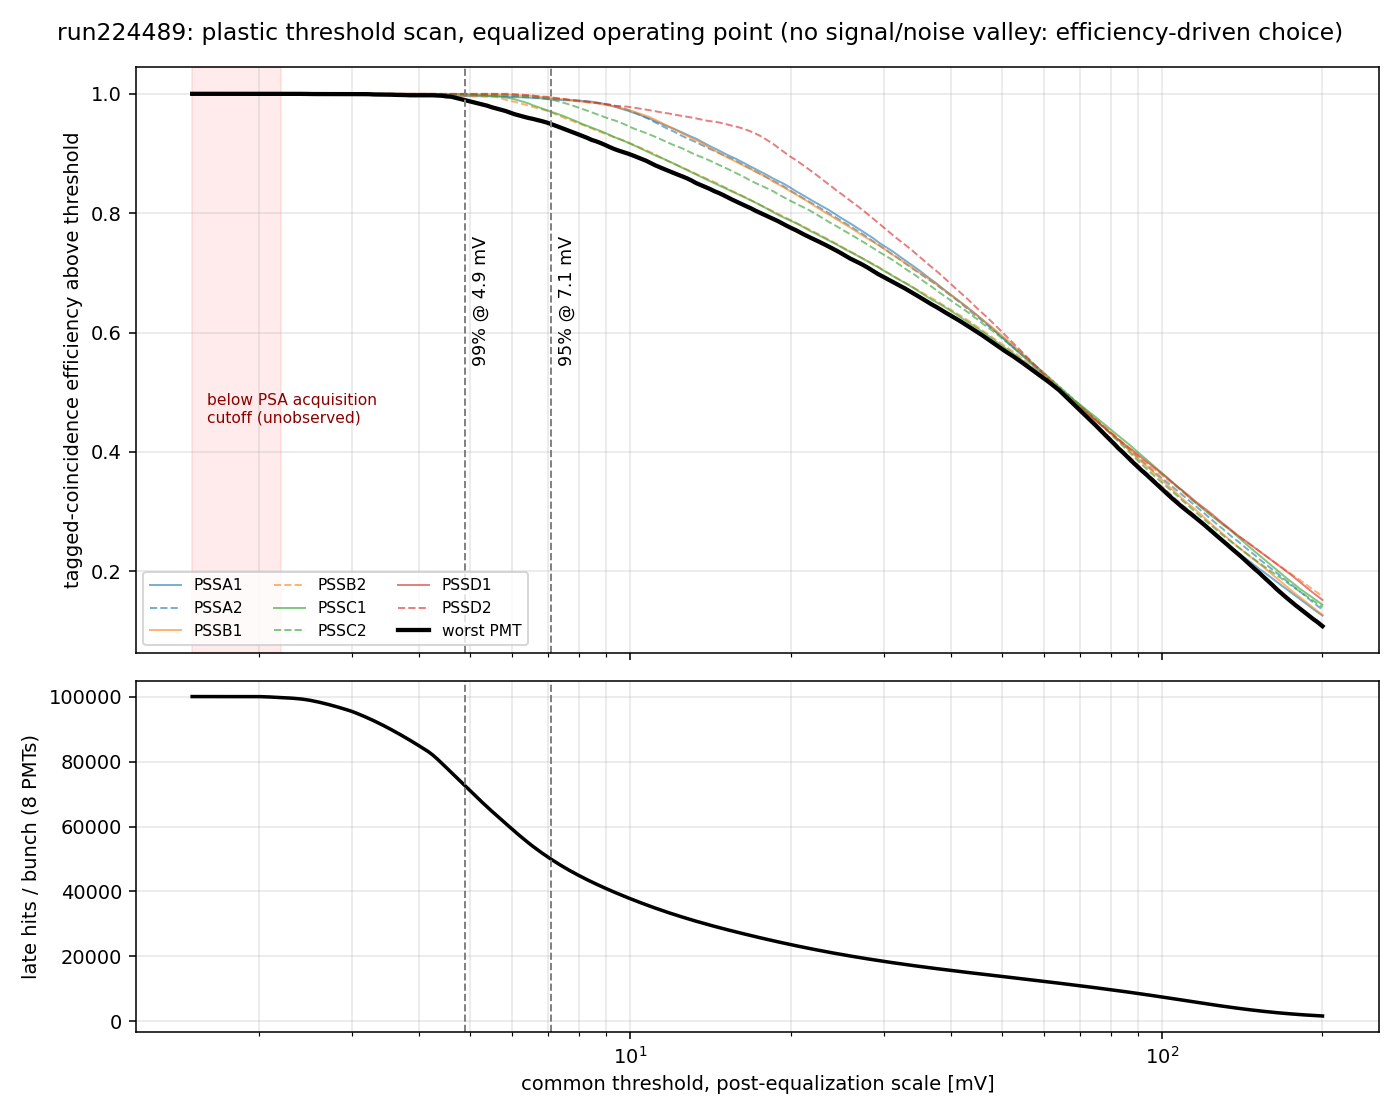
\includegraphics[width=.8\textwidth]{12_hv_scan/threshold_scan.png}
\caption{Common-threshold scan at equalized gains.}
\label{fig:threshold}
\end{figure}

\section{The liquids: timed in on every arm}
\label{sec:liqtime}
The LIQ channels had never been timed. A wide ($\pm400$\,ns) coincidence scan
against the same-arm wall and plastic finds a sharp peak on every arm
(Fig.~\ref{fig:liqwide}): the LIQ pulse \emph{leads} the plastic by
29.5--32.8\,ns and sits within $\pm3.3$\,ns of the wall. Per-channel offsets
(8 wall channels $\times$ arm, plus both plastic bars; rms 3.2--4.5\,ns) are
written to \texttt{calib/liq\_offsets\_run224489.json} --- a new file, so no
existing consumer of the wall--plastic offsets breaks
(Fig.~\ref{fig:liqtiming}).

\begin{figure}[H]\centering
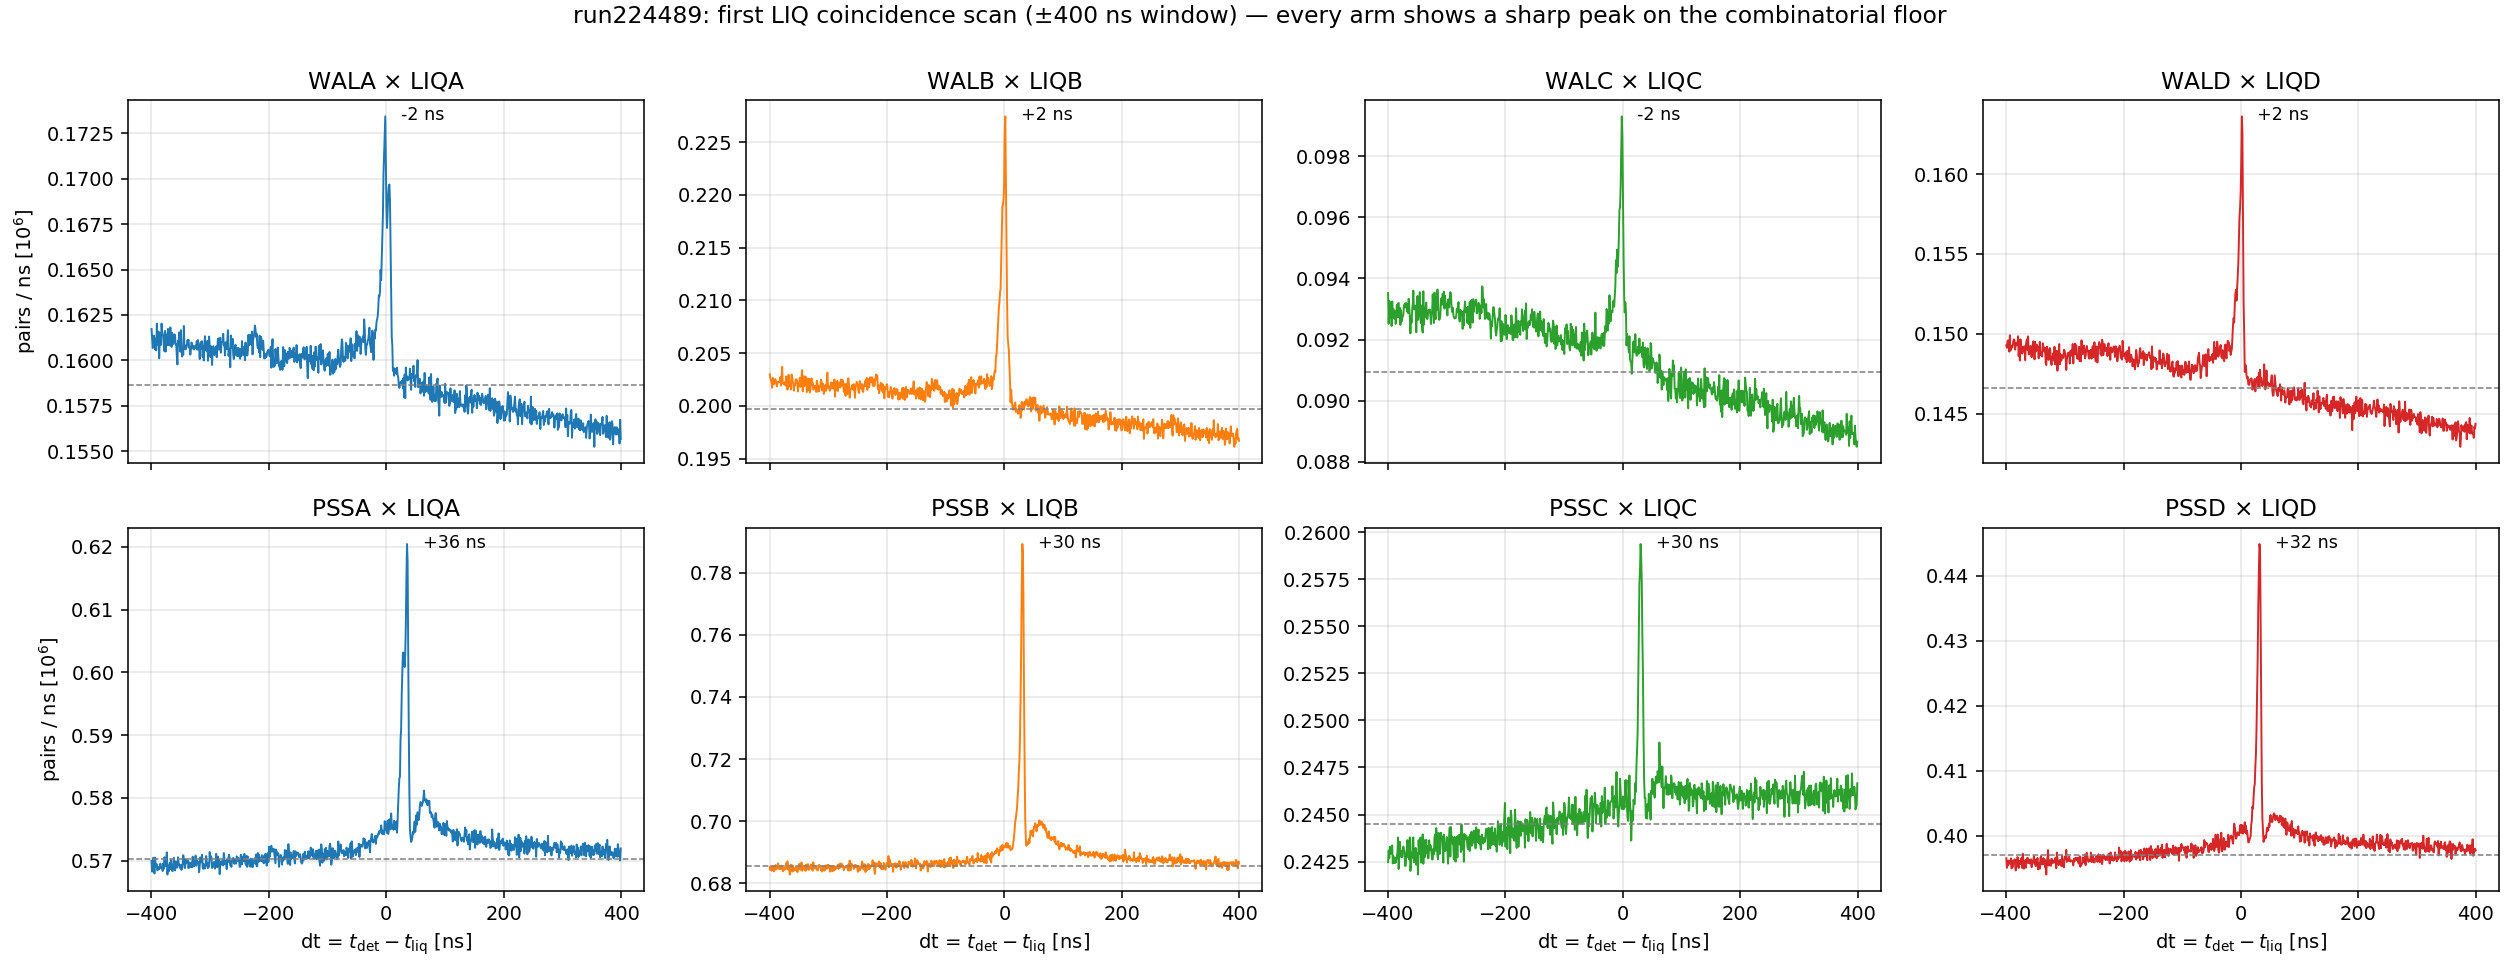
\includegraphics[width=\textwidth]{19_triples/liq_wide_dt.png}
\caption{First LIQ coincidence scan, $\pm400$\,ns: WAL$\times$LIQ (top) and
PSS$\times$LIQ (bottom) per arm.}
\label{fig:liqwide}
\end{figure}

\begin{figure}[H]\centering
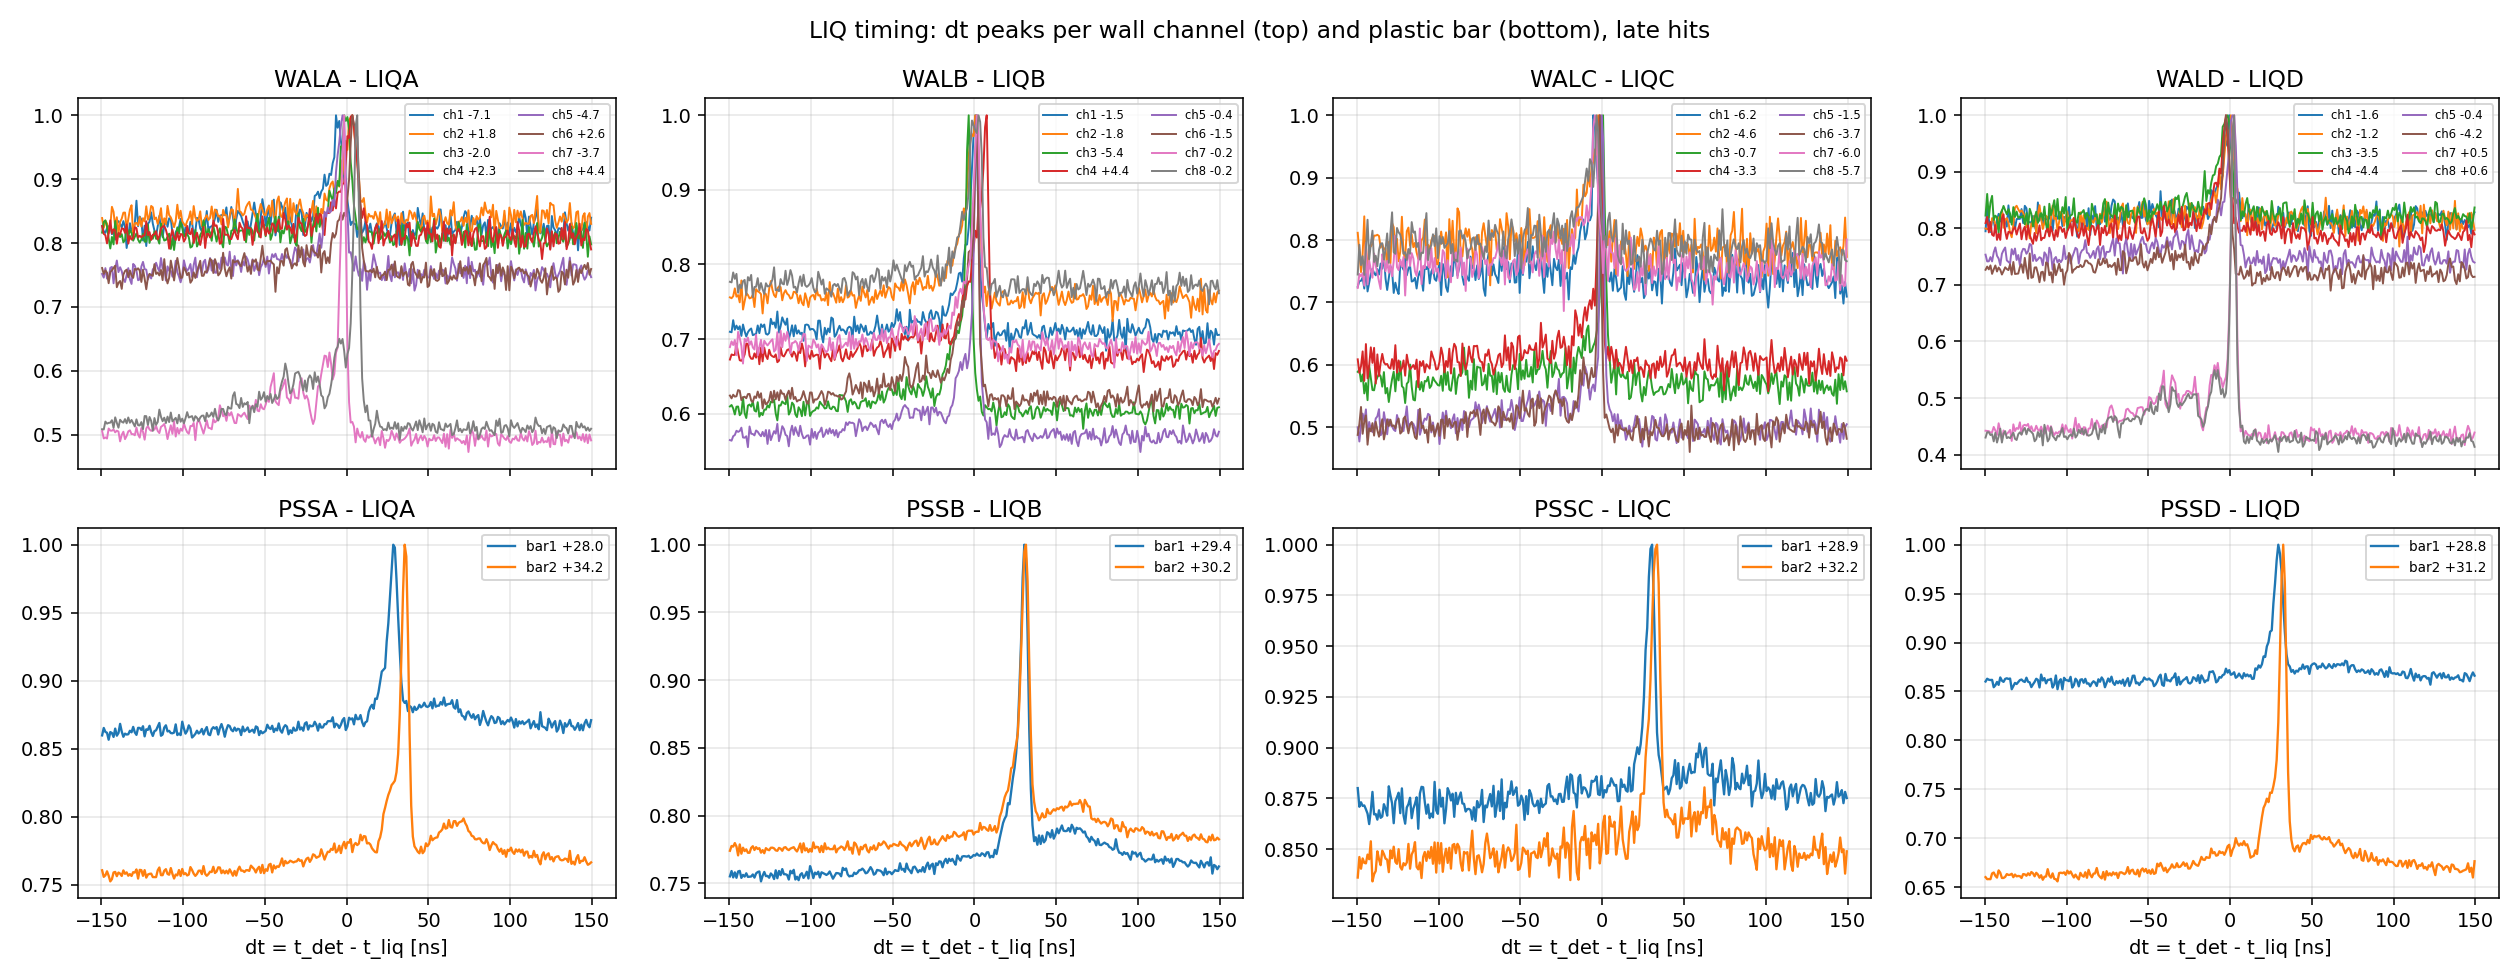
\includegraphics[width=\textwidth]{19_triples/liq_timing.png}
\caption{LIQ timing peaks per wall channel (top row) and per plastic bar
(bottom row).}
\label{fig:liqtiming}
\end{figure}

\section{Triple coincidences: the first plastic MIP}
\label{sec:triples}
A wall--plastic coincidence MIP-tags only the \emph{wall} (the plastic is
behind the wall, so its spectrum in pairs is just a hit spectrum). With the
liquids live, a third tag behind the plastic closes the telescope: the
as-built stack is MM $\to$ SiPM wall $\to$ plastics $\to$ single LS layer, so
a WAL$\times$PSS$\times$LIQ triple selects through-going particles and the
\emph{plastic} spectrum in triples is a genuine MIP-candidate spectrum
(Fig.~\ref{fig:concept}).

\begin{figure}[H]\centering
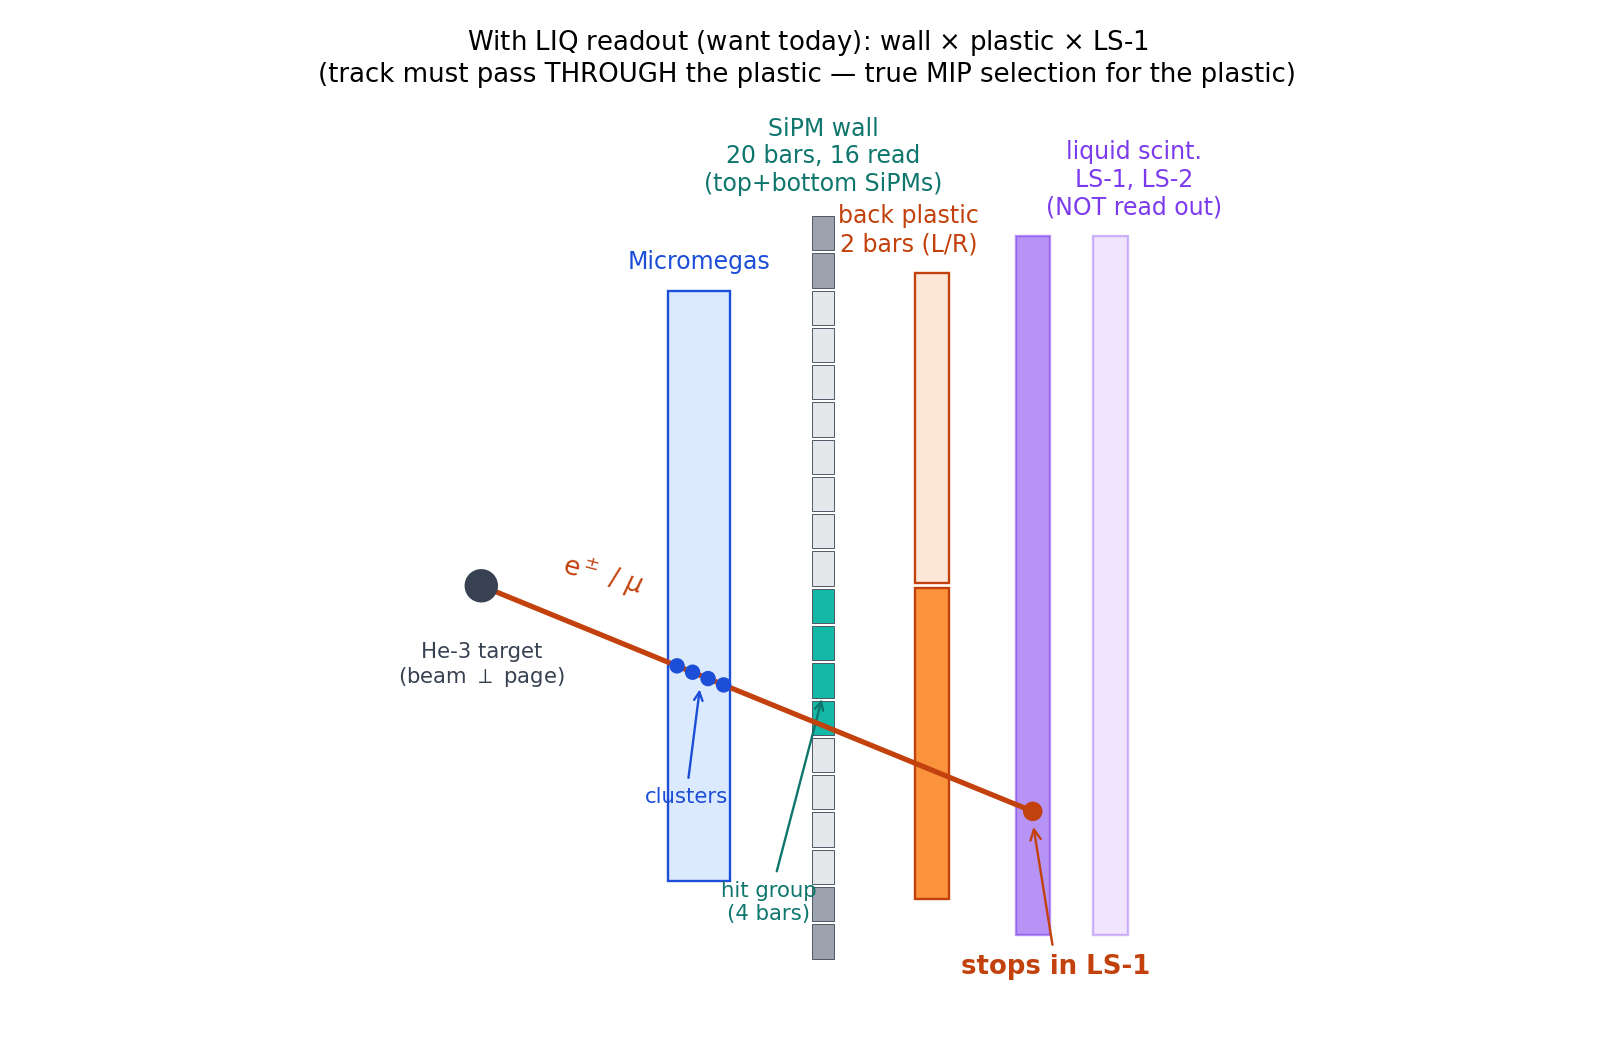
\includegraphics[width=.7\textwidth]{11_diagrams/concept_wall_plastic_liq.png}
\caption{The triple-coincidence telescope.}
\label{fig:concept}
\end{figure}

Triples are built from wall--plastic pairs ($|dt_{\rm cal}|\leq8$\,ns after
the new offsets; sideband $+20$..$+120$\,ns) matched to LIQ hits near the
plastic time ($|dt_{\rm LIQ}|\leq10$\,ns around the per-arm peak; double
sideband $25$--$125$\,ns both sides), and every spectrum is double
sideband-subtracted in both $dt$'s. Net triple counts per PMT range from
9.2\,k (CL) to 49.5\,k (BR) --- but split over the HV steps this is only
$\sim$2--6\,k per PMT per step, so the individual per-step spectra
(Fig.~\ref{fig:mipspectra}) are statistically noisy; they show the spectral
hump marching with HV but are not, by themselves, compelling.

The compelling test is gain alignment (Fig.~\ref{fig:mipaligned}): scaling
each step's spectrum to its nominal-voltage equivalent (a multiplication by
$(V_{\rm nom}/V)^{n}$, i.e.\ a pure translation in log amplitude) must make a
\emph{physical} peak coincide across steps, while the fixed-ADC threshold
edge moves from step to step. That is exactly what the data do: the aligned
steps pile up at a common position and their sum --- one high-statistics
spectrum per PMT --- shows a single dominant peak at the adopted MIP value,
3--6$\times$ above even the worst step's aligned threshold edge. A threshold
artifact cannot produce this behavior. (The aligned stacks also reveal a
genuine secondary component at $\sim$100--300\,mV equivalent, most visible on
AR/BR/DR --- large energy deposits, composition not yet identified.) As a
further systematic check, adding the LIQ tag leaves the \emph{wall} spectrum
in triples unchanged (Fig.~\ref{fig:wallintriples}): the third tag purifies
without biasing.

\begin{figure}[H]\centering
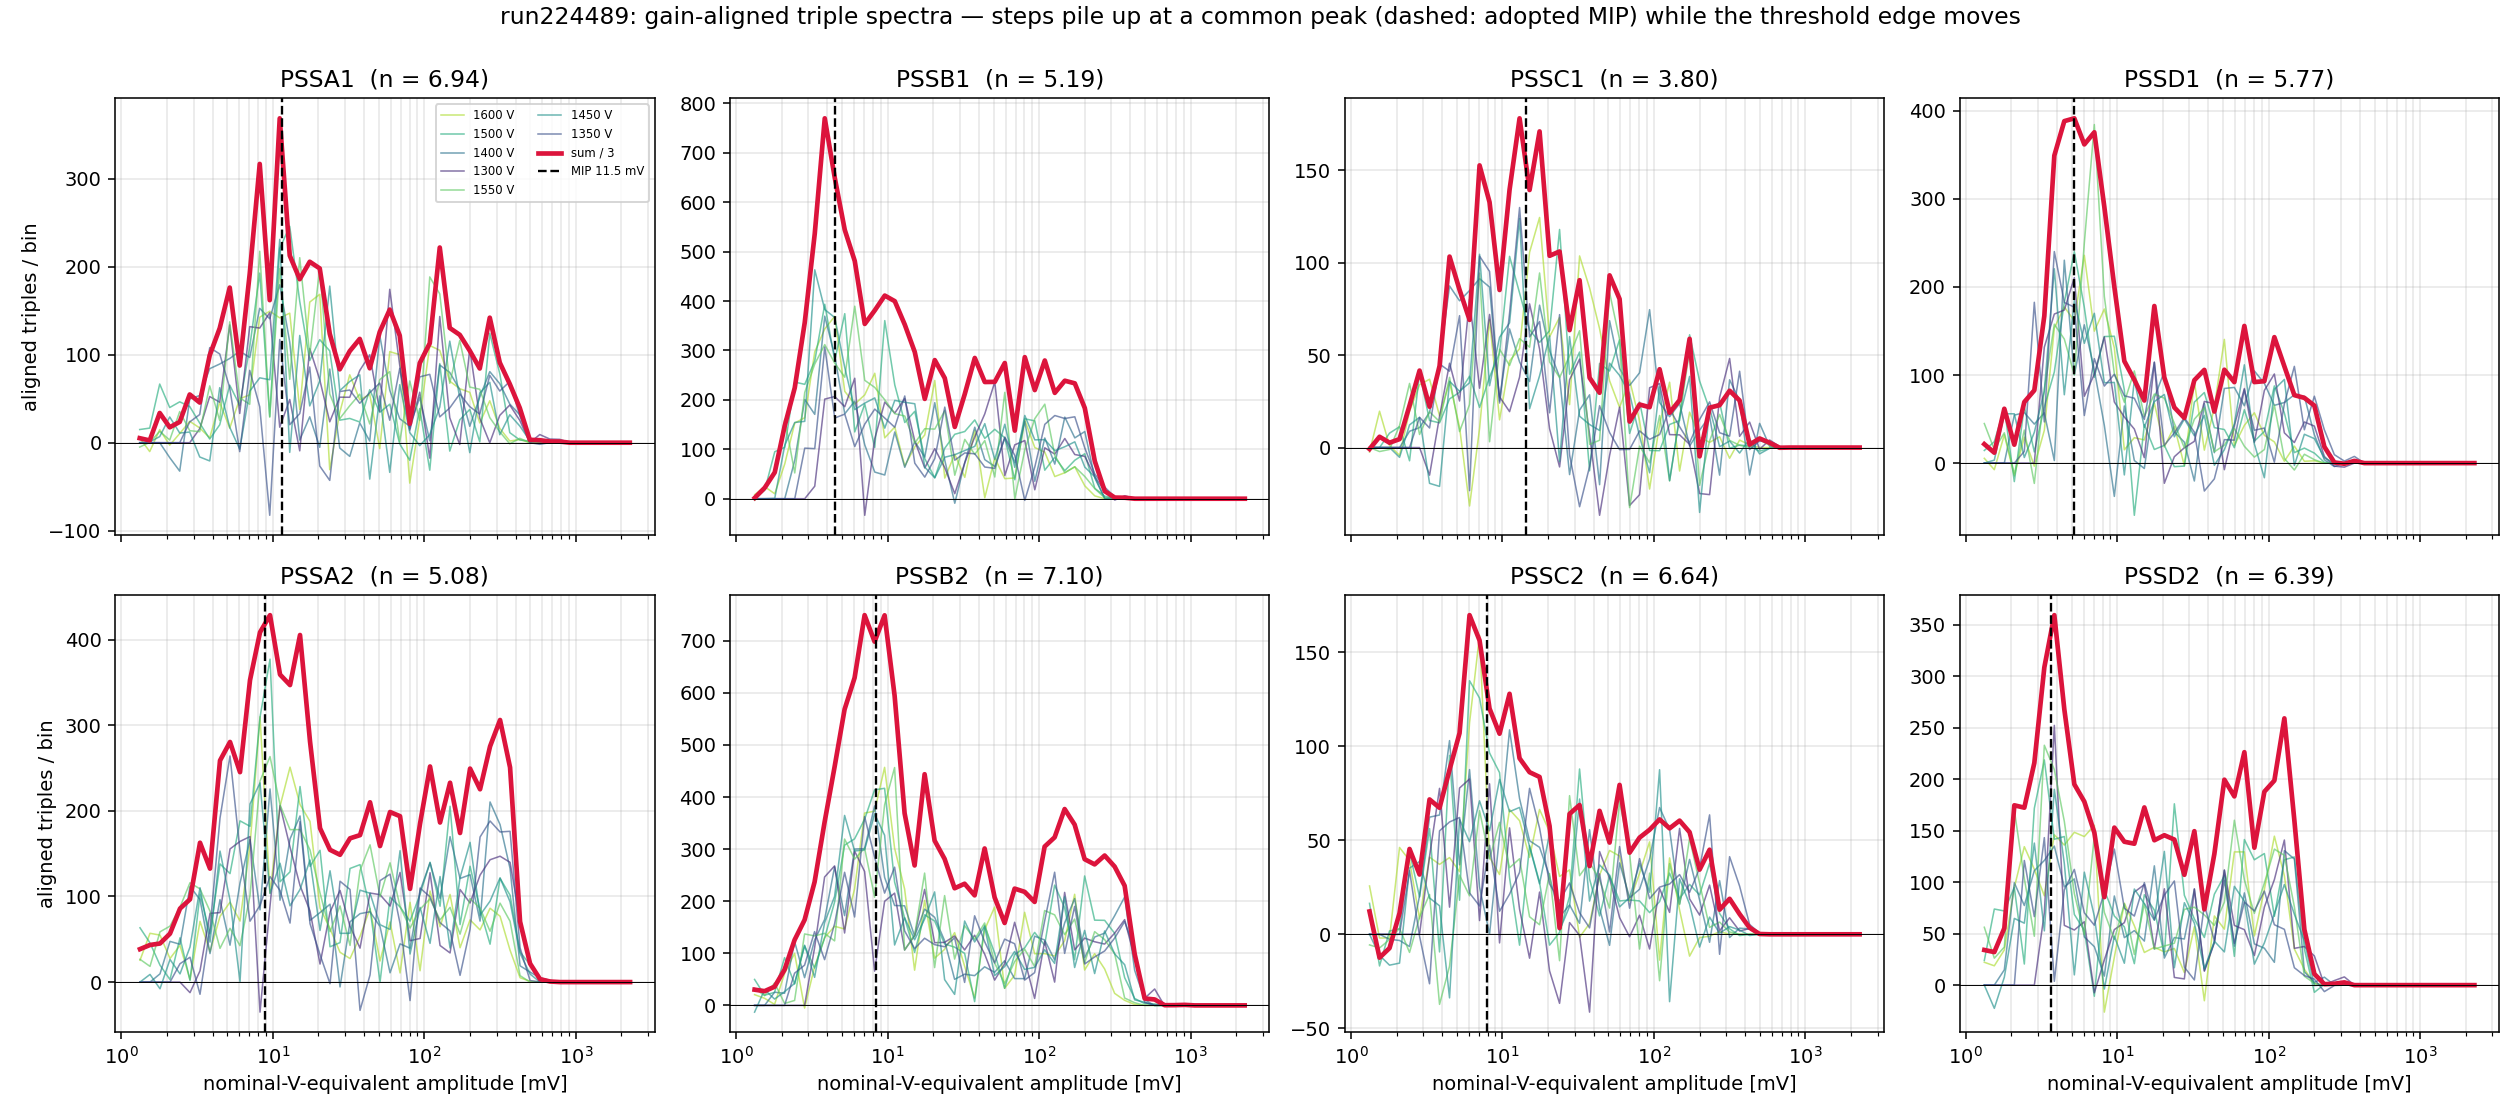
\includegraphics[width=\textwidth]{19_triples/pss_mip_aligned.png}
\caption{Gain-aligned triple-tagged plastic spectra: thin curves are
individual steps ($V\geq1300$\,V) scaled to nominal-V equivalent, the red
curve is their sum ($/3$), the dashed line the adopted MIP. A physical peak
aligns; the threshold edge does not.}
\label{fig:mipaligned}
\end{figure}

\begin{figure}[H]\centering
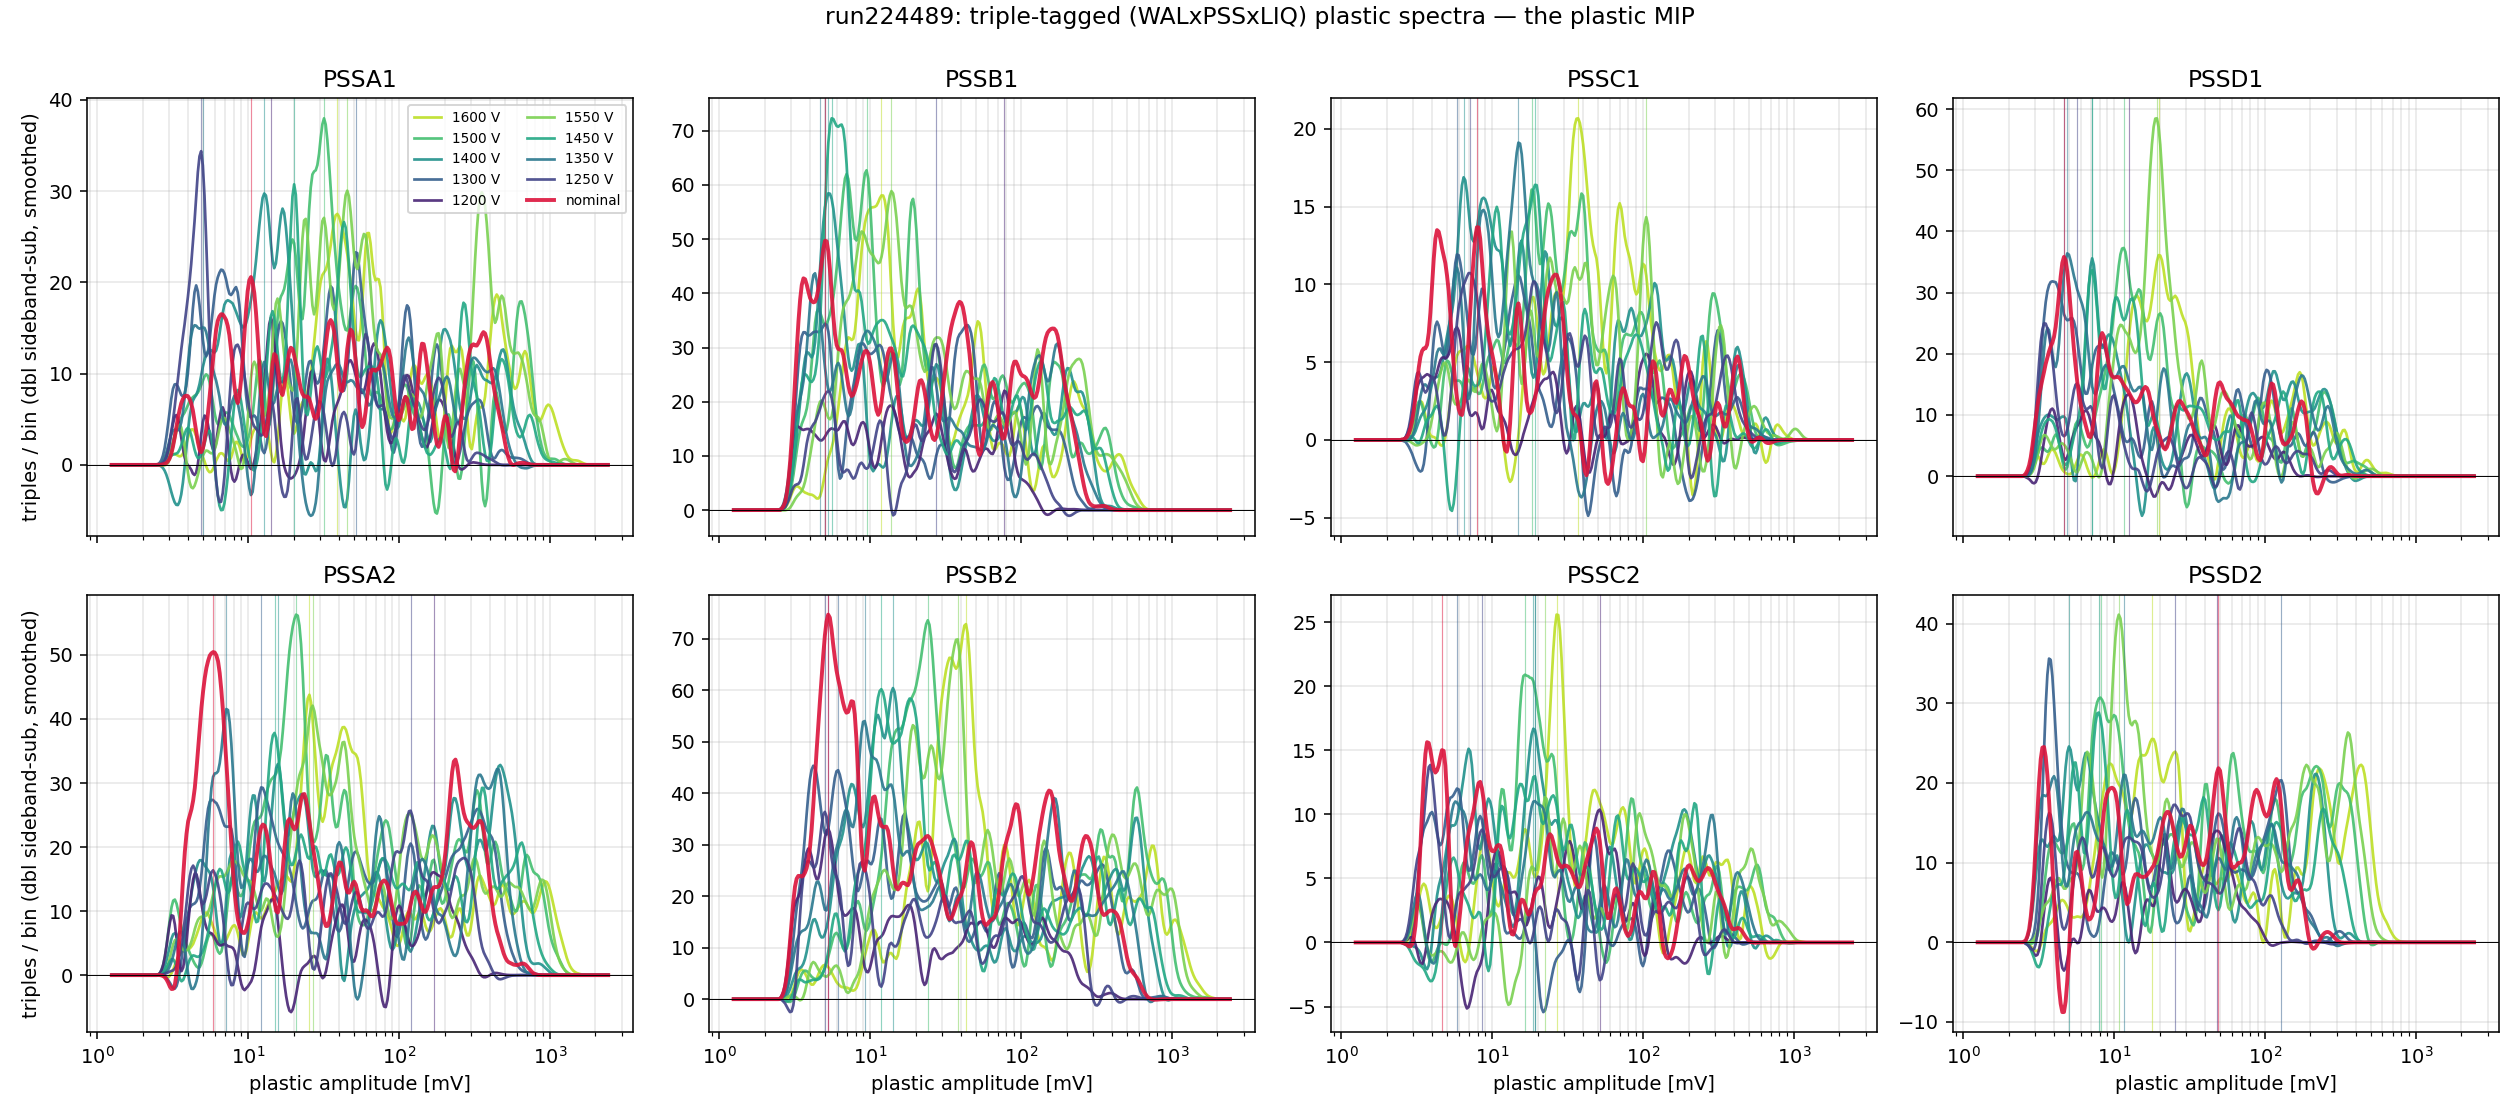
\includegraphics[width=\textwidth]{19_triples/pss_mip_spectra.png}
\caption{Triple-tagged plastic spectra per HV step (double
sideband-subtracted, rebinned $\times$6; readable subset of steps shown).
The MIP hump moves coherently with HV; the red curve is the nominal-HV
window.}
\label{fig:mipspectra}
\end{figure}

\begin{figure}[H]\centering
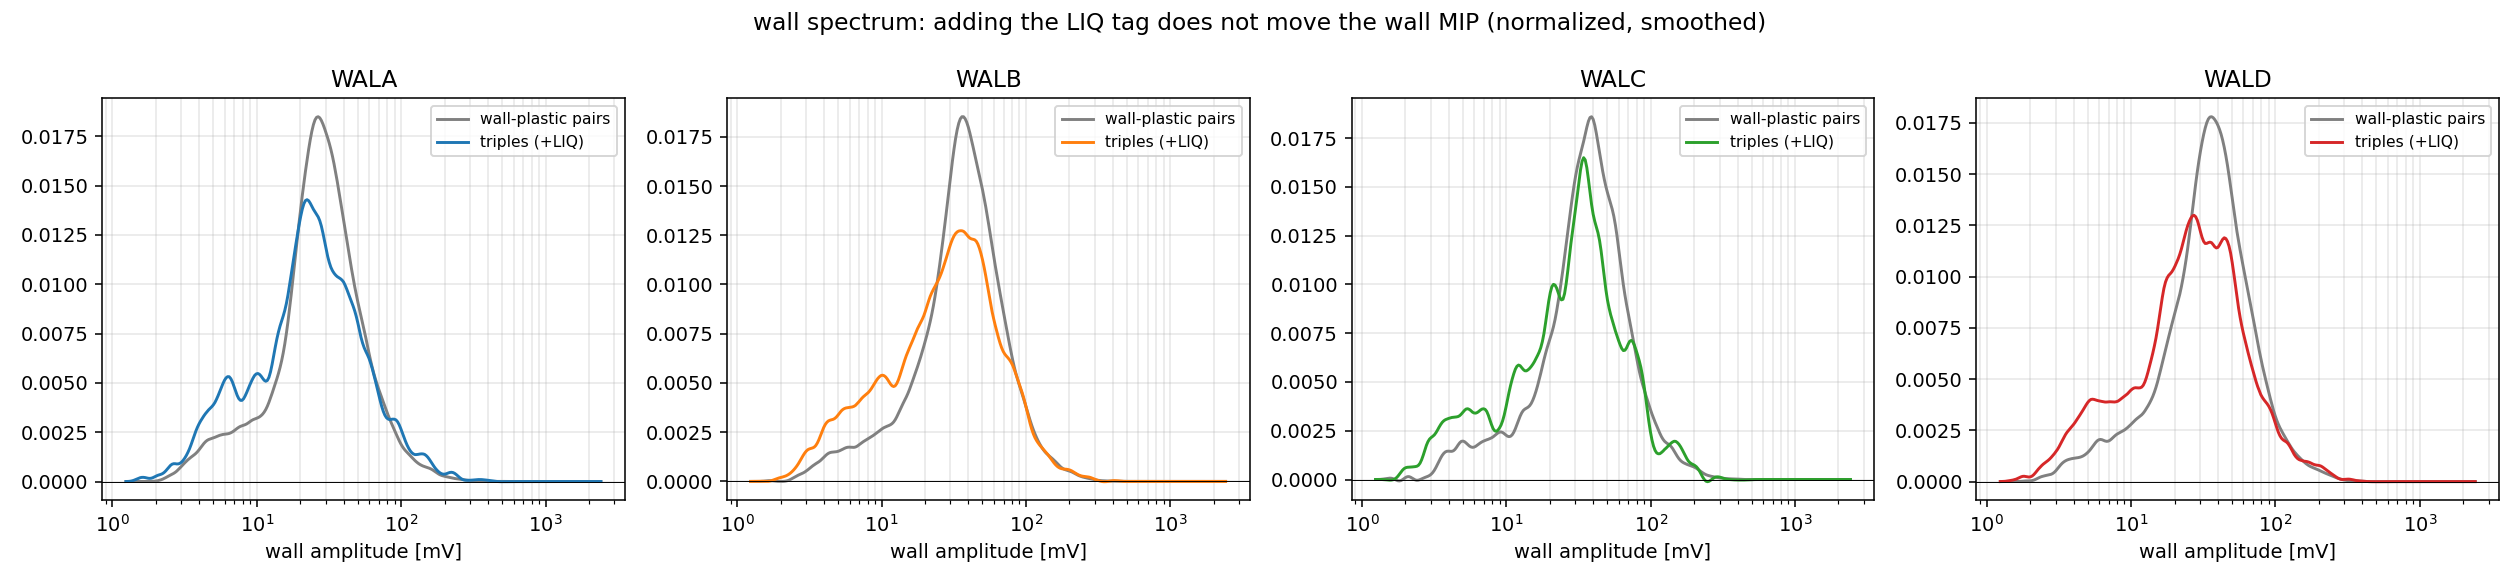
\includegraphics[width=\textwidth]{19_triples/wall_in_triples.png}
\caption{Wall spectra in wall--plastic pairs vs.\ triples (normalized): the
LIQ tag does not move the wall MIP.}
\label{fig:wallintriples}
\end{figure}

The clearest view is one HV step per panel on a \emph{linear} amplitude axis
with coarse bins and propagated Poisson errors
(Figs.~\ref{fig:stepsBR}--\ref{fig:stepsDR}; all eight PMTs in
\texttt{figures/19\_triples/steps\_linear/}): a single peak, significant
against its error bars, tracking the power-law expectation panel after panel
while the fixed acquisition threshold (gray) stays put. These linear spectra
also exposed a convention bias in the first-pass numbers: the mode of a
log-binned spectrum ($dN/d\log A = A\,dN/dA$) sits systematically 20--40\%
above the true linear-space MPV of $dN/dA$, which is the quantity a Landau
MPV convention means. The adopted calibration is therefore the peak of the
\emph{gain-aligned summed} linear spectrum (every $V\geq1400$\,V step scaled
to its nominal-V equivalent and summed --- one $\sim$15\,k-triple spectrum
per PMT), located with a lightly smoothed peak finder; the statistical error
is the standard deviation of the peak over Poisson bootstraps of the four
sideband components, and the per-step scatter (Table~\ref{tab:mip}
``spread'') measures transport consistency. At these statistics different
reasonable peak estimators genuinely differ by 10--30\% on the weaker PMTs
--- that spread, not the bootstrap error alone, is the honest uncertainty of
this first calibration.

The decisive trust check is Fig.~\ref{fig:mipvsv}: the per-step MIP MPVs
plotted against the \emph{no-MIP-selection} pair-coincident median (the
$\sim$100$\times$-statistics gain proxy from the HV scan). Both follow the
same power law in $V$ --- parallel lines in log-log, $n_{\rm MIP}$ consistent
with $n_{\rm median}$ within the low-stats fit errors --- with the MIP
sitting a factor 8--15 below the median (physical: the pair-tagged plastic
spectrum is dominated by larger deposits than a through-going MIP). A noise
artifact would not scale with HV like a gain.

\begin{figure}[H]\centering
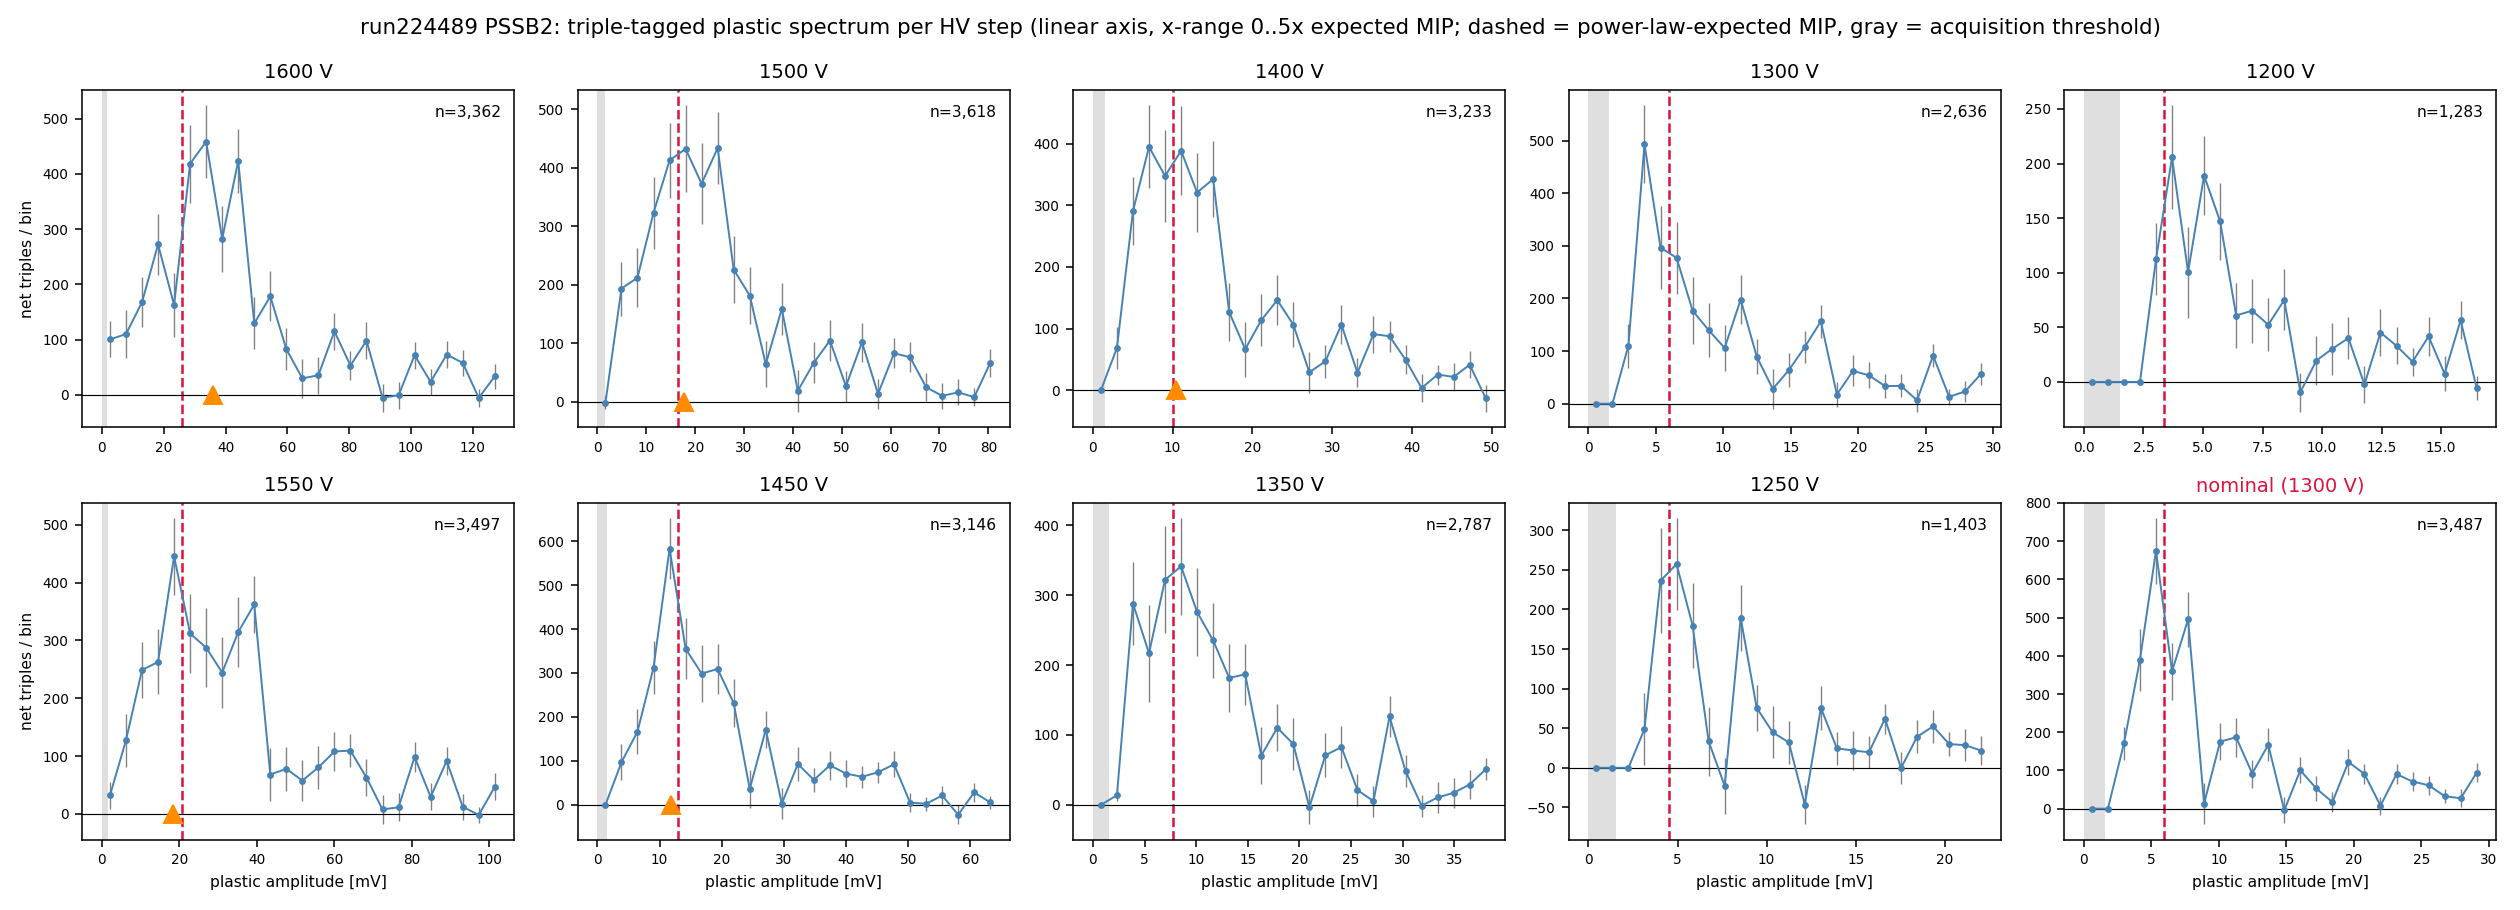
\includegraphics[width=\textwidth]{19_triples/steps_linear/mip_steps_PSSB2.png}
\caption{PSSB2: triple-tagged plastic spectrum, one HV step per panel, linear
amplitude axis, propagated errors. Dashed: power-law-expected MPV; orange
triangle: per-step fitted MPV; gray band: acquisition threshold.}
\label{fig:stepsBR}
\end{figure}

\begin{figure}[H]\centering
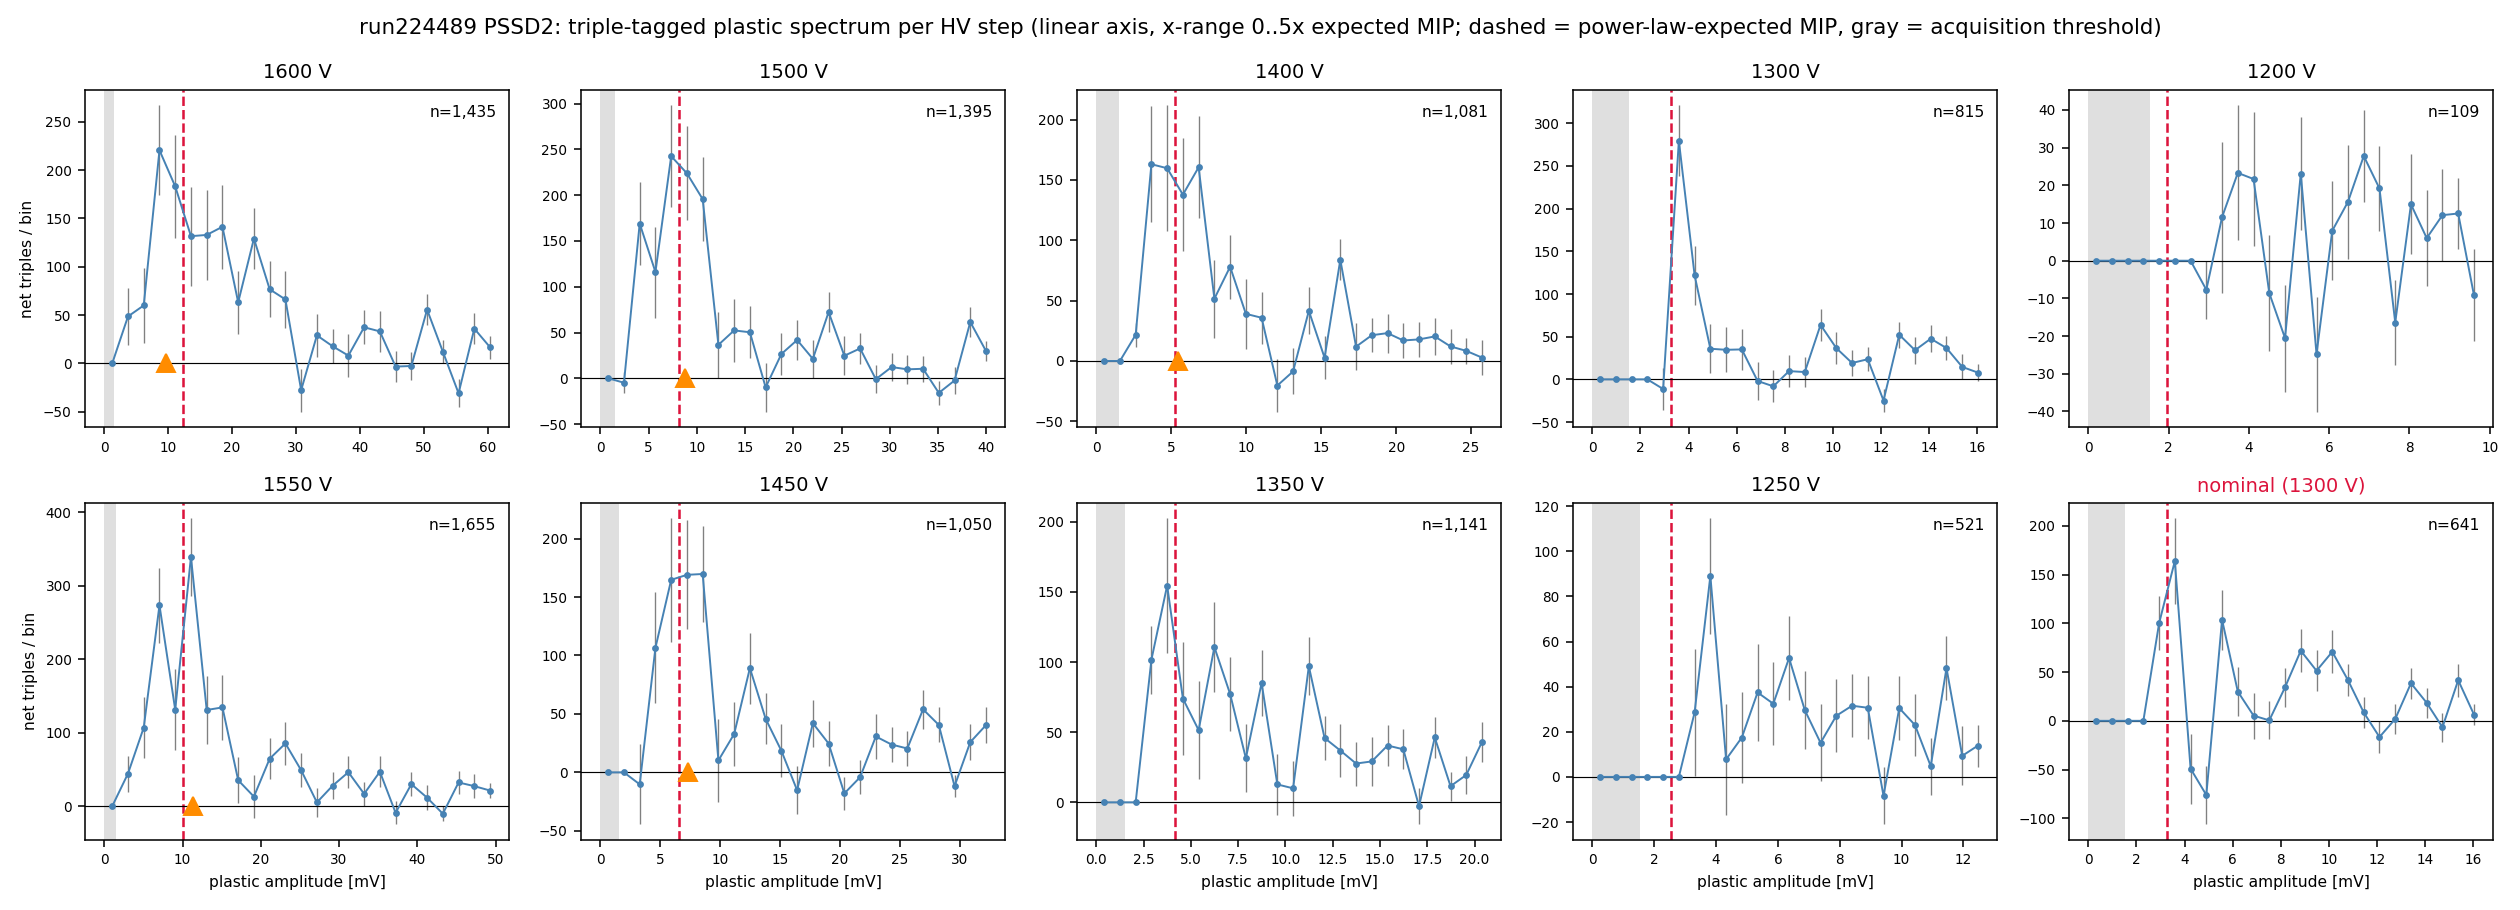
\includegraphics[width=\textwidth]{19_triples/steps_linear/mip_steps_PSSD2.png}
\caption{Same for PSSD2, the lowest-gain PMT: the peak is clear at
$V\geq1400$\,V but rides the threshold at low HV and at nominal --- which is
why only $V\geq1400$\,V enters the fit, and why this arm cannot trigger on
plastic MIPs at the current HV.}
\label{fig:stepsDR}
\end{figure}

\begin{figure}[H]\centering
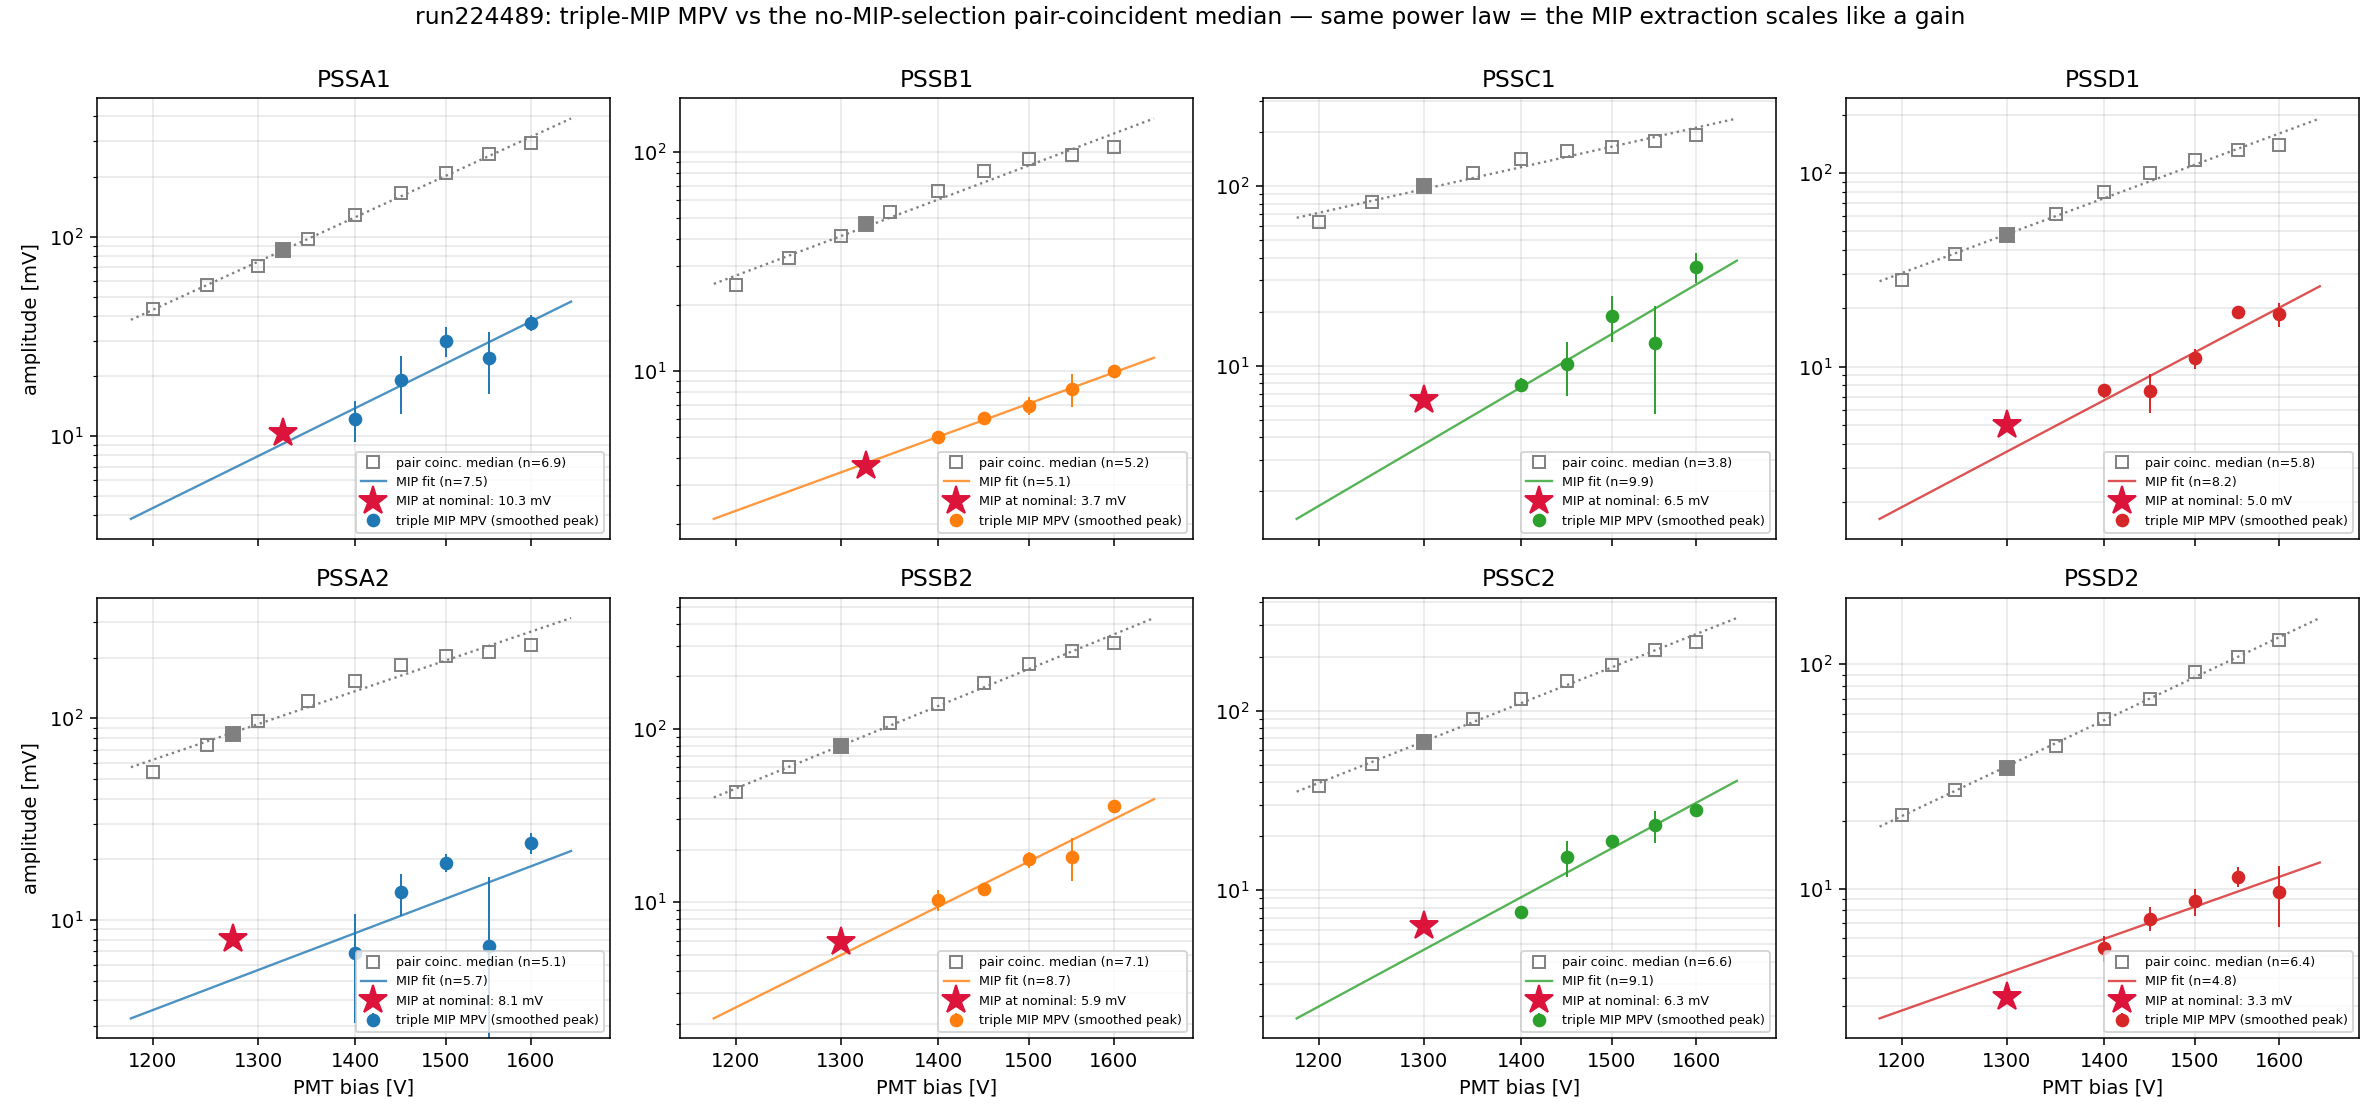
\includegraphics[width=\textwidth]{19_triples/mip_vs_v_median_compare.png}
\caption{Per-step triple-MIP MPVs (colored, bootstrap errors, own power-law
fit) vs.\ the pair-coincident median without any MIP selection (gray squares,
dotted fit; filled square = nominal-HV window). Star: the adopted aligned-sum
MPV at nominal HV. Same slope $=$ the MIP extraction scales like a gain.}
\label{fig:mipvsv}
\end{figure}

\begin{table}[H]\centering\small
\begin{tabular}{lrrrrr}
\toprule
PMT & $V_{\rm nom}$ [V] & $n$ & MPV [mV] & spread & mV/MeV\\
\midrule
PSSA1 (AL) & 1325 & 6.94 & $10.3\pm1.5$ & 16\% & 2.05\\
PSSA2 (AR) & 1275 & 5.08 & $ 8.1\pm1.2$ & 42\% & 1.60\\
PSSB1 (BL) & 1325 & 5.19 & $ 3.7\pm0.5$ &  2\% & 0.73\\
PSSB2 (BR) & 1300 & 7.10 & $ 5.9\pm0.5$ & 16\% & 1.18\\
PSSC1 (CL) & 1300 & 3.80 & $ 6.5\pm1.6$ & 38\% & 1.28\\
PSSC2 (CR) & 1300 & 6.64 & $ 6.3\pm0.3$ & 18\% & 1.25\\
PSSD1 (DL) & 1300 & 5.77 & $ 5.0\pm0.6$ & 18\% & 0.99\\
PSSD2 (DR) & 1300 & 6.39 & $ 3.3\pm0.3$ & 14\% & 0.65\\
\bottomrule
\end{tabular}
\caption{Plastic MIP (linear-space MPV) at nominal HV and absolute
calibration. MPV from the gain-aligned summed spectrum with bootstrap
statistical error; ``spread'' is the per-step transport scatter (the fuller
uncertainty on the weaker PMTs). The energy scale assumes the
normal-incidence minimum-ionizing deposit in 2.5\,cm of PVT
($1.956\,\mathrm{MeV\,cm^2/g}\times1.032\,\mathrm{g/cm^3}\times2.5\,\mathrm{cm}
= 5.05$\,MeV); the incidence-angle path-length spread ($\sim$+10--20\% on the
mean) is not yet corrected. \texttt{calib/pss\_mip\_calib\_run224489.json}
(the earlier log-binned-mode values are preserved there as
\texttt{mip\_mv\_logmode}).}
\label{tab:mip}
\end{table}

Two operational consequences. First, the MIP-based inter-PMT gain ratios
agree with the coincident-median equalization to $\sim$15\%, an independent
validation of Table~\ref{tab:eq}. Second, and important for the trigger:
\textbf{at the current HV the DR (3.3\,mV) and BL (3.7\,mV) MIPs are
below the 4.9\,mV threshold} that the threshold scan recommends --- those arms
cannot trigger efficiently on plastic MIPs until the equalization
($+133$/$+84$\,V) is applied.

\section{LIQ gain vs.\ position: the gradient is real}
\label{sec:liqpos}
The triple sample also locates each through-going track: horizontally by wall
group (4 bins) and plastic bar (2), vertically by the top/bottom SiPM
asymmetry $\ln(A_{\rm top}/A_{\rm bot})$ of the tagged wall hit (6 bins).
Accumulating the LIQ amplitude in these bins (all double sideband-subtracted)
gives Fig.~\ref{fig:liqpos}. The marginal profiles are unambiguous:

\begin{itemize}
\item \textbf{A and D} (vessels HORIZONTAL, PMT toward wall group 4): the
      horizontal profile rises from 9.1$\to$17.5\,mV (A) and
      6.4$\to$11.1\,mV (D) toward group 4, while the vertical profile is
      flat.
\item \textbf{B and C} (vessels VERTICAL, PMT up): the vertical profile rises
      toward the top (11.7$\to$17.5\,mV on B, 4.5$\to$7.8\,mV on C), while
      the horizontal profile is mild.
\end{itemize}

A 1.5--2$\times$ light-collection gradient along the vessel axis, higher near
the PMT, whose direction flips exactly with the surveyed vessel orientation
(vertical PMT-up on B/C, horizontal PMT-along-$+u$ on A/D in the as-built
Geant geometry). Any LIQ energy interpretation needs a position correction,
which the triple machinery can now supply. The LIQ pulse-height scale itself
is uncomfortably low on C and D (inclusive medians 4.7 and 5.3\,mV vs.\
10.4\,mV on B): LIQ HV/gain review is advisable alongside the plastic
equalization (Fig.~\ref{fig:liqspec}).

\begin{figure}[H]\centering
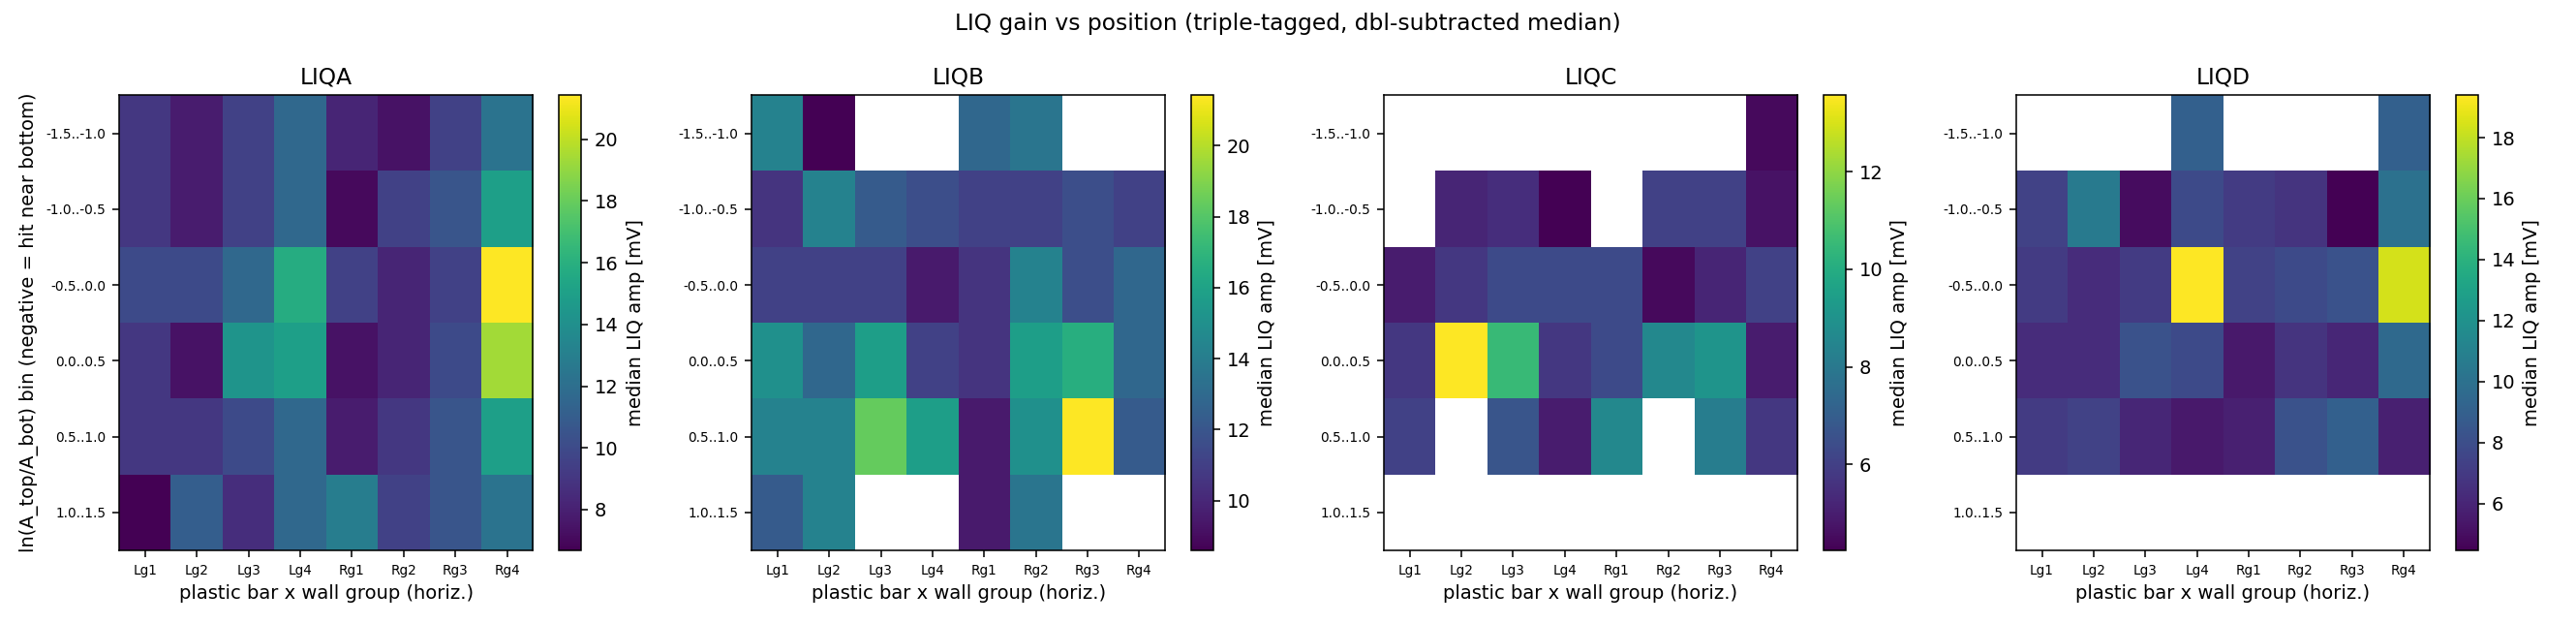
\includegraphics[width=\textwidth]{19_triples/liq_position_map.png}
\caption{Median LIQ amplitude per position bin (triple-tagged, double
sideband-subtracted). Columns: plastic bar $\times$ wall group (left$\to$right
as seen from the back); rows: vertical asymmetry bins (negative = hit near
the bottom).}
\label{fig:liqpos}
\end{figure}

\begin{figure}[H]\centering
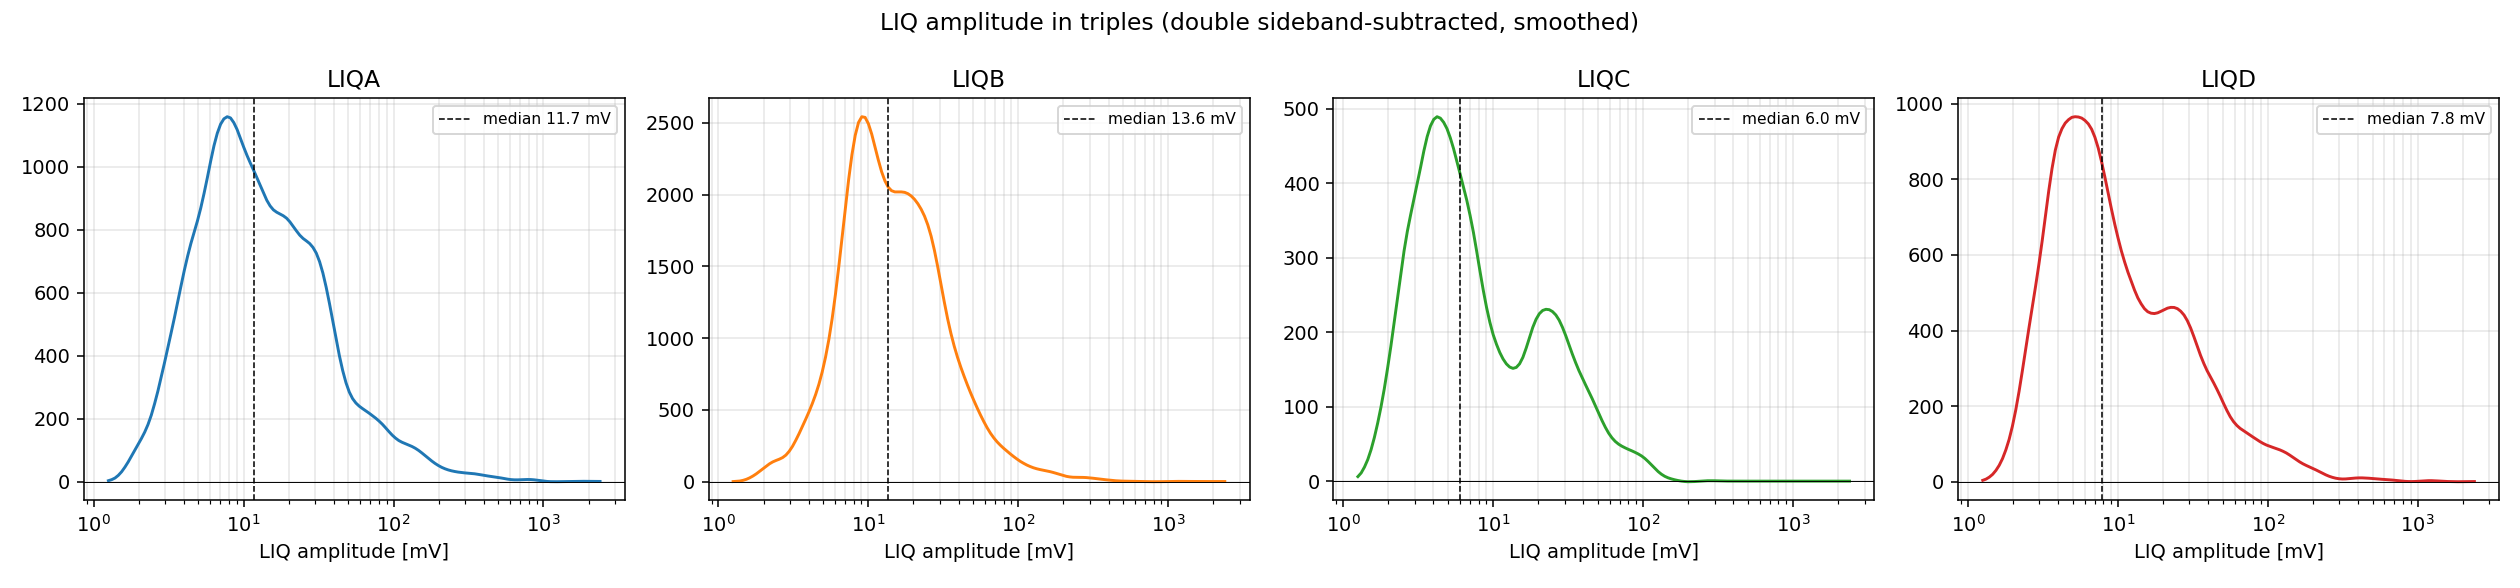
\includegraphics[width=\textwidth]{19_triples/liq_spectra.png}
\caption{Triple-tagged LIQ amplitude spectra per arm.}
\label{fig:liqspec}
\end{figure}

\section{Timing program}
\label{sec:timing}
\textbf{Common offset shift.} The new per-channel wall--plastic offsets
(\texttt{calib/time\_offsets\_run224489.json}) differ from the 224466 ones by
a single common $-22.27$\,ns with 0.22\,ns rms across all 64 channel pairs
(Fig.~\ref{fig:offshift}) --- the FIFO path is a clean common delay
(somewhat larger than the $\geq$16\,ns cable estimate), and the sign matches
``plastics later $\Rightarrow$ $dt=t_{\rm wall}-t_{\rm pss}$ more negative''.

\begin{figure}[H]\centering
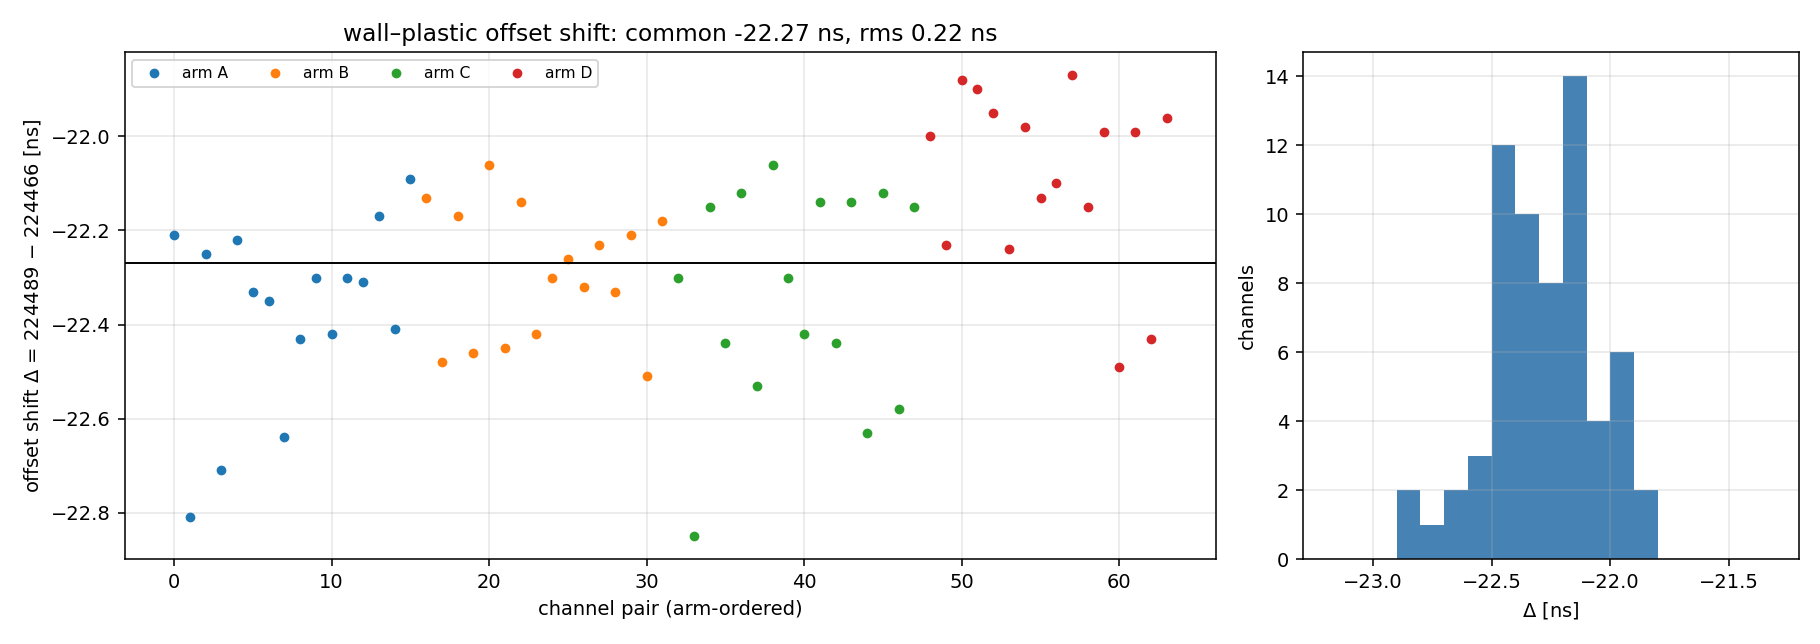
\includegraphics[width=.95\textwidth]{19_triples/offset_shift.png}
\caption{Per-channel offset shift between runs.}
\label{fig:offshift}
\end{figure}

\textbf{The $-60$\,ns satellite is not a plastic-cable reflection.} In 224466
the late-tof B/C dt spectra showed a small satellite at $dt\approx-60$\,ns
(6--9\% of the main peak). If it were a reflection or afterpulse tied to the
plastic signal path, the $-22$\,ns path change would move it with the main
peak. Instead it kept its \emph{absolute} position ($-60$ to $-68$\,ns) while
the main peak moved by $-22$\,ns --- and it grew to 19--34\% of the main peak
(Fig.~\ref{fig:satellite}). Both facts point at something injected at or
after the FIFO (digitizer side), and the growth suggests the FIFO itself
participates. It stays outside all signal and sideband windows, so no result
here is affected, but a scope check at the FIFO outputs is recommended.

\begin{figure}[H]\centering
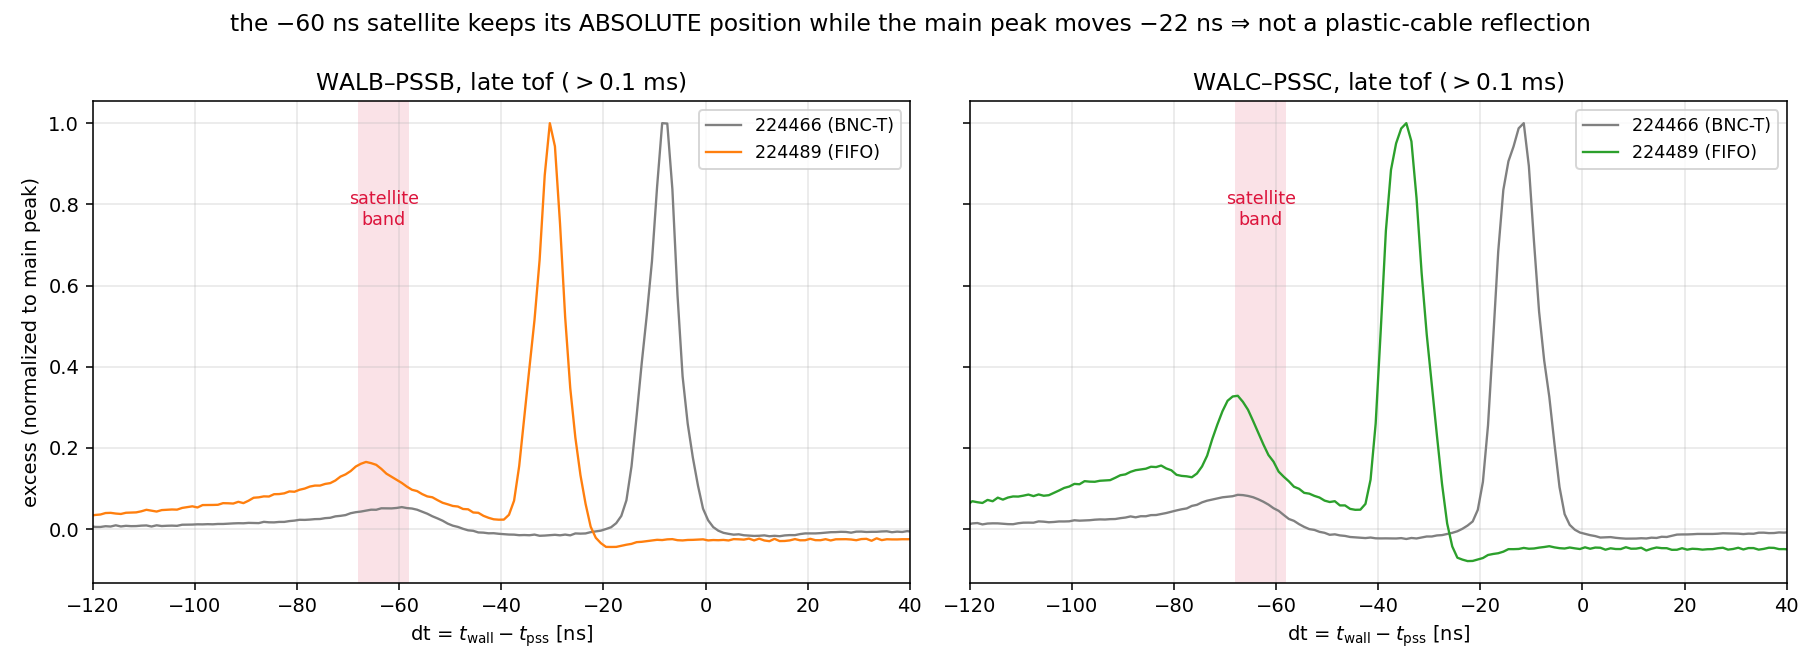
\includegraphics[width=.95\textwidth]{19_triples/satellite.png}
\caption{Late-tof dt spectra, normalized to the main peak, both runs.}
\label{fig:satellite}
\end{figure}

\section{Summary and recommendations}
\begin{enumerate}
\item The A/D cross-wiring is fixed and fully explains the old A/D
      coincidence deficit; the wall MIP calibration now covers all four arms.
\item The plastic MIP is measured for the first time:
      0.65--2.05\,mV/MeV at nominal HV. \textbf{Apply the new equalization}
      (Table~\ref{tab:eq}); until then DR and BL cannot trigger on plastic
      MIPs at the recommended 4.9\,mV threshold.
\item Use the measured per-PMT FIFO ratios ($\times$1.13--1.65), not a
      global $\times2$, in any comparison with pre-FIFO data.
\item The liquids are timed in (offsets published); the LIQ position-gain
      gradient (1.5--2$\times$, toward the PMT) must be corrected before any
      LIQ energy use; C/D LIQ gains look low --- review LIQ HV.
\item Scope-check the FIFO outputs for the $-60$\,ns satellite, which tripled
      in relative size with the new path.
\end{enumerate}

\vspace{1ex}
\noindent\textit{Reproducibility: caches and calibrations are keyed by run
stem under \texttt{mx\_july\_beam\_qa/} (\texttt{cache/*\_run224489.npz},
\texttt{calib/*\_run224489.json}); triples machinery in
\texttt{19\_liq\_triples.py} (+\texttt{19b}, \texttt{19c}); HV-scan step
tables per run in \texttt{12\_plastic\_hv\_scan.py}.}

\end{document}
